% (c) 2012 -2014 Dimitrios Vrettos - d.vrettos@gmail.com

\chapter{Disequazioni}

\section{Intervalli sulla retta reale}

\begin{definizione}
 Dati due numeri reali~$a$ e~$b$, con~$a<b$, si chiamano
\emph{intervalli} i seguenti sottoinsiemi di~$\insR$:

\begin{enumeratea}
\item $(a\text{,~}b)=\left\{x\in \insR\mid a<x<b\right\}$ intervallo \emph{limitato} \emph{aperto} ($a$ e~$b$ sono esclusi)\footnote{gli intervalli aperti possono anche essere indicati con la parentesi quadra opposta. Ad esempio l'intervallo $(a\text{,~}b)$ può essere anche scritto $]a\text{,~}b[$, come $[a\text{,~}b)$ può essere scritto $[a\text{,~}b[$.};
\item $[a\text{,~}b]=\left\{x\in \insR\mid a\le x\le b\right\}$ intervallo \emph{limitato} \emph{chiuso} ($a$ e~$b$ sono inclusi);
\item $[a\text{,~}b)=\left\{x\in \insR\mid a\le x<b\right\}$ intervallo \emph{limitato} \emph{chiuso a sinistra} e \emph{aperto a destra} ($a$ è incluso e $b$ è escluso);
\item $(a\text{,~}b]=\left\{x\in \insR\mid a<x\le b\right\}$ intervallo \emph{limitato} \emph{aperto a sinistra} e \emph{chiuso a destra} ($a$ è escluso e $b$ è incluso);
\item $(a\text{,~}+\infty)=\left\{x\in\insR\mid x>a\right\}$ intervallo \emph{superiormente illimitato} \emph{aperto} ($a$ è escluso);
\item $[a\text{,~}+\infty)=\left\{x\in \insR\mid x\ge a\right\}$ intervallo \emph{superiormente illimitato} \emph{chiuso a sinistra} ($a$ è incluso);
\item $(-\infty\text{,~}b)=\left\{x\in\insR\mid x<b\right\}$ intervallo \emph{inferiormente illimitato} \emph{aperto} ($b$ è escluso);
\item $(-\infty\text{,~}b]=\left\{x\in \insR\mid x\le b\right\}$ intervallo \emph{inferiormente illimitato} \emph{chiuso a destra} ($b$ è escluso).
\end{enumeratea}

I numeri~$a$ e~$b$ si chiamano \emph{estremi} (rispettivamente \emph{inferiore} e \emph{superiore})
dell'intervallo.
\end{definizione}

I numeri reali $\insR$ possono essere messi in corrispondenza biunivoca con i
punti di una retta: ogni numero reale ha per immagine un punto della
retta e viceversa ogni punto della retta è immagine di un numero
reale. Di conseguenza ognuno degli intervalli sopra definiti ha per
immagine una semiretta o un segmento, precisamente gli intervalli
limitati corrispondono a segmenti e quelli illimitati a semirette.
Vediamo con degli esempi come si rappresentano i diversi tipi di
intervalli sulla retta $r$ immagine dei valori reali.

\begin{exrig}
 \begin{esempio}
 $H=\{x\in \insR\mid x<3\}$ intervallo illimitato inferiormente:~$H=(-\infty\text{,~}3)$.
 \end{esempio}

 L'insieme~$H$ è rappresentato da tutti i punti della
semiretta che precedono il punto immagine del numero~3, esclusa
l'origine della semiretta (3). Nella figura, la semiretta
dei punti che appartengono ad~$H$ è stata disegnata con una linea più
spessa e di colore differente. Per mettere in evidenza che il punto immagine di~3 non
appartiene alla semiretta abbiamo messo un pallino vuoto sul punto.
\begin{center}
 % (c) 2012 Dimitrios Vrettos - d.vrettos@gmail.com
\begin{tikzpicture}[font=\small,x=10mm, y=5mm]

\draw[->] (0,0) -- (8,0) node [below right] () {$r$};
\node[above]  at (4,0) {3};
\begin{scope}[blue,thick]
\draw (0,0) -- (4,0);
\draw[fill=white] (4,0)circle (1.5pt);
\end{scope}

\end{tikzpicture}
\end{center}

 \begin{esempio}
 $P=\{x\in \insR\mid x\ge -5\}$ intervallo
illimitato superiormente chiuso a sinistra: $P=[-5\text{,~}+\infty)$.
 \end{esempio}

Segniamo sulla retta~$r$ il punto immagine di~$-5$;
l'insieme~$P$ è rappresentato dalla semiretta di tutti
i punti che seguono~$-5$, compreso lo stesso~$-5$. Nel disegno, la
semiretta dei punti che appartengono a~$P$ è stata disegnata con una
linea più spessa e di colore differente. Per indicare che il punto~$-5$ appartiene
all'intervallo abbiamo messo un pallino pieno sul punto.
\begin{center}
 % (c) 2012 Dimitrios Vrettos - d.vrettos@gmail.com
\begin{tikzpicture}[font=\small,x=10mm, y=5mm]

\draw[->] (0,0) -- (8,0) node [below right] () {$r$};
\node[above]  at (4,0) {$-5$};
\begin{scope}[blue,thick,->]
\draw (4,0) -- (8,0);
\draw[fill=blue] (4,0)circle (1.5pt);
\end{scope}

\end{tikzpicture}
\end{center}

 \begin{esempio}
 $D=\{x\in \insR\mid -2<x<6\}$ intervallo limitato aperto:~$D=(-2\text{,~}6)$.
 \end{esempio}

Segniamo sulla retta reale i punti immagine degli estremi del segmento,
$-2$ e~$6$. L'insieme~$D$ è rappresentato dal segmento che
ha per estremi questi due punti. Nel disegno il segmento è stato
disegnato con una linea più spessa e di colore differente. I due estremi del segmento sono
esclusi, pertanto su ciascuno di essi abbiamo messo un pallino vuoto.
\begin{center}
 % (c) 2012 Dimitrios Vrettos - d.vrettos@gmail.com
\begin{tikzpicture}[font=\small,x=10mm, y=5mm]

\draw[->] (0,0) -- (8,0) node [below right] () {$r$};
\node[above]  at (1,0) {$-2$};
\node[above]  at (7,0) {6};
\begin{scope}[blue,thick]
\draw (1,0) -- (7,0);
\foreach \x in {1,7}
\draw[fill=white] (\x,0)circle (1.5pt);
\end{scope}

\end{tikzpicture}
\end{center}

 \begin{esempio}
 $T=\{x\in \insR\mid -2<x\le~6\}$ intervallo limitato chiuso a destra:~$T=(-2\text{,~}6]$.
 \end{esempio}

Rispetto al caso precedente, il segmento che rappresenta
l'insieme~$T$ è chiuso a destra, ossia è incluso
nell'intervallo anche il suo estremo superiore~($6$), mentre è escluso il suo estremo inferiore~($-2$).
\begin{center}
 % (c) 2012 Dimitrios Vrettos - d.vrettos@gmail.com
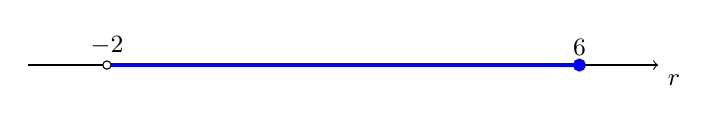
\begin{tikzpicture}[font=\small,x=10mm, y=5mm]

\draw[->] (0,0) -- (8,0) node [below right] () {$r$};
\node[above]  at (1,0) {$-2$};
\node[above]  at (7,0) {6};
\begin{scope}[blue,ultra thick]
\draw (1,0) -- (7,0);
\draw[fill=blue] (7,0)circle (1.5pt);
\end{scope}
\draw[fill=white] (1,0)circle (1.5pt);

\end{tikzpicture}
\end{center}

 \begin{esempio}
 $S=\{x\in \insR\mid -2\le x\le~6\}$ intervallo chiuso e limitato:~$S=[2\text{,~}6]$.
 \end{esempio}

Il segmento che rappresenta l'insieme~$S$ contiene tutti e
due i suoi estremi.
\begin{center}
 % (c) 2012 Dimitrios Vrettos - d.vrettos@gmail.com
\begin{tikzpicture}[font=\small,x=10mm, y=5mm]

\draw[->] (0,0) -- (8,0) node [below right] () {$r$};
\node[above]  at (1,0) {$-2$};
\node[above]  at (7,0) {6};
\begin{scope}[blue,thick]
\draw (1,0) -- (7,0);
\foreach \x in {1,7}
\draw[fill=blue] (\x,0)circle (1.5pt);
\end{scope}

\end{tikzpicture}
\end{center}

 \begin{esempio}
 Altri particolari sottoinsiemi dei numeri reali sono:
 \end{esempio}

\begin{itemize}
\item $\insR^{+}=\{x\in \insR\mid x>0\}$. Semiretta di origine~0 costituita da tutti i
numeri reali positivi:
\begin{center}
 % (c) 2012 Dimitrios Vrettos - d.vrettos@gmail.com
\begin{tikzpicture}[font=\small,x=10mm, y=5mm]

\draw[->] (0,0) -- (8,0) node [below right] () {$r$};
\node[above]  at (4,0) {0};
\begin{scope}[blue,thick,->]
\draw (4,0) -- (8,0);
\draw[fill=white] (4,0)circle (1.5pt);
\end{scope}

\end{tikzpicture}
\end{center}
\item $\insR^{-}=\{x\in \insR\mid x<0\}$. Semiretta di origine~0 costituita da tutti i numeri reali negativi:
\begin{center}
 % (c) 2012 Dimitrios Vrettos - d.vrettos@gmail.com
\begin{tikzpicture}[font=\small,x=10mm, y=5mm]

\draw[->] (0,0) -- (8,0) node [below right] () {$r$};
\node[above]  at (4,0) {0};
\begin{scope}[blue,thick]
\draw (0,0) -- (4,0);
\draw[fill=white] (4,0)circle (1.5pt);
\end{scope}

\end{tikzpicture}
\end{center}
\subitem Il punto~0 non appartiene a nessuna delle due semirette poiché il numero~0
non appartiene né a~$\insR^{+}$ né a~$\insR^{-}$:~$\insR=\insR^{+}\cup\insR^{-}\cup\{0\}$.

\item $\insR_{0}^{+}=\{x\in \insR\mid x\ge~0\}$;
\item $\insR_{0}^{-}=\{x\in \insR\mid x\le~0\}$.
\end{itemize}
\end{exrig}

\ovalbox{\risolvii \ref{ese:20.1}, \ref{ese:20.2}, \ref{ese:20.3}, \ref{ese:20.4}, \ref{ese:20.5}, \ref{ese:20.6}, \ref{ese:20.7}}

\section{Disequazioni numeriche}
Consideriamo le seguenti proposizioni:

\begin{enumeratea}
\item 5 è minore di~12;
\item $48-90$ è maggiore di~30;
\item il quadrato di un numero reale è maggiore o uguale a zero;
\item sommando ad un numero la sua metà si ottiene un numero minore
o uguale a~1.
\end{enumeratea}

Esse possono essere tradotte in linguaggio matematico usando i simboli
$>$ (maggiore), $<$~(minore), ${\ge}$ (maggiore o uguale), ${\le}$ (minore o uguale) e precisamente:

\begin{multicols}{4}
 \begin{enumeratea}
\item $5<12$;
\item $48-90>30$;
\item $x^{2}\ge~0$;
\item $x+\frac{1}{2}x\le~1$.
 \end{enumeratea}
\end{multicols}

Le formule che contengono variabili si dicono \emph{aperte}; quelle che
contengono solo numeri si dicono \emph{chiuse}. Quindi a) e b) sono formule
chiuse; c) e d) sono formule aperte.

\begin{definizione}
 Chiamiamo \emph{disuguaglianza} una formula chiusa
costruita con uno dei predicati~$<$ (essere minore),
$>$ (essere maggiore), ${\le}$ (essere minore o uguale),
${\ge}$ (essere maggiore o uguale).
\end{definizione}

Di essa sappiamo subito stabilire il valore di verità, quando è
stabilito l'ambiente in cui vengono enunciate.

\begin{definizione}
Chiamiamo \emph{disequazione} una formula aperta,
definita in~$\insR$ e costruita con uno dei seguenti predicati:~$<$
(essere minore), $>$ (essere maggiore), ${\leq}$
(essere minore o uguale), ${\geq}$ (essere
maggiore o uguale).
\end{definizione}

Analogamente a quanto detto per le equazioni, chiamiamo
\emph{incognite} le variabili che compaiono nella disequazione,
\emph{primo membro} e \emph{secondo membro} le due espressioni che
compaiono a sinistra e a destra del segno di disuguaglianza.

\begin{exrig}
 \begin{esempio}
 Disuguaglianze vere e false.

 \begin{enumeratea}
\item in~$\insN$, la formula~$5>0$ è una disuguaglianza vera;
\item in~$\insZ$, la formula~$-6>-4$ è una disuguaglianza falsa;
\item la formula~$5x>0$ è una disequazione; quando
all'incognita sostituiamo un numero essa si trasforma
in una disuguaglianza e solo allora possiamo stabilirne il valore di
verità. Nel caso proposto è vera se sostituiamo
alla variabile un qualunque numero positivo, falsa se
sostituiamo zero o un numero negativo.
\end{enumeratea}
 \end{esempio}

\end{exrig}

\ovalbox{\risolvi \ref{ese:20.8}}

\begin{definizione}
L'insieme dei valori che sostituiti all'incognita trasformano
la~disequazione in una
disuguaglianza vera, è l'\emph{insieme soluzione} ($\IS$) della disequazione.
\end{definizione}

\subsection{Ricerca dell'insieme soluzione di una disequazione}

Alcune volte l'$\IS$ si può trovare
ragionando sulla forma della disequazione.

 \begin{exrig}
  \begin{esempio}
   Analizziamo le seguenti disequazioni in~$\insR$:


\begin{itemize}
\item $3\cdot x\ge~0$. Si cercano quei valori da attribuire
all'incognita che moltiplicati per~3 diano un prodotto
positivo o nullo. Per le regole dei segni e per la legge di
annullamento del prodotto, il numero~$x$ deve essere maggiore o uguale
a~0:~$\IS=\{x\in \insR\mid x\ge~0\}=\insR^{+}\cup\{0\}=\insR^{+}_0$;
\item $x^{2}+1<0$. Si cercano i valori che rendono la somma del loro
quadrato con~1 un numero negativo. Poiché il quadrato di un numero
è sempre positivo, al più nullo se il numero è zero, aggiungendo
ad esso~1, non troveremo mai un risultato negativo:~$\IS=\emptyset $;
\item $-x^{2}\le~0$. Il primo membro è l'opposto del
quadrato di un numero; poiché il quadrato è sempre positivo o
nullo, la disequazione è verificata per qualunque numero reale:~$\IS=\insR$;
\item $\dfrac{1}{x}<0$. Il primo membro è l'inverso di
un numero reale; tale operazione ha significato per qualunque numero
tranne che per~0, $\dfrac{1}{0}$ infatti è priva di significato. La
frazione~$\dfrac{1}{x}$ è negativa per qualunque valore negativo
attribuito all'incognita $x$: $\IS=\{x\in\insR\mid x<0\}=\insR^{-}$.
\end{itemize}
  \end{esempio}
 \end{exrig}

In questo paragrafo affronteremo disequazioni in una sola incognita,
che, dopo aver svolto eventuali calcoli nei due membri, avranno
l'incognita al primo grado e i cui coefficienti sono
numeri reali.

La forma più semplice o \emph{forma canonica} di una disequazione di
primo grado in una sola incognita a coefficienti reali è una delle
seguenti~$ax>b$; $ax<b$; $ax\ge b$; $ax\le b$ (con~$a$ e~$b$ numeri reali).

Per ridurre una disequazione alla forma canonica e quindi per
determinare il suo~$\IS$ si procede applicando dei principi analoghi a
quelli delle equazioni.

Premettiamo la seguente definizione:

\begin{definizione}
Due disequazioni si dicono \emph{equivalenti} se hanno lo
stesso insieme delle soluzioni.
\end{definizione}

\begin{principio}[I Principio]
\label{ppd}
Addizionando o sottraendo a ciascuno dei due membri di
una disequazione uno stesso numero o una
stessa espressione (definita per qualunque
valore attribuito all'incognita), si ottiene una
disequazione equivalente alla data.
\end{principio}

Regola pratica: questo principio ci permette di
``spostare'' un addendo da un membro
all'altro cambiandogli segno o di
``eliminare'' da entrambi i membri
gli addendi uguali.

\begin{principio}[II Principio]
Moltiplicando o dividendo ciascuno dei due membri di
una disequazione per uno stesso numero positivo o per
una stessa espressione (definita e positiva
per qualunque valore attribuito alla variabile), si ottiene una
disequazione equivalente alla data.
\end{principio}


\begin{principio}[III Principio]
Moltiplicando o dividendo ciascuno dei due membri di
una disequazione per uno stesso numero negativo o per
una stessa espressione (definita e negativa
per qualunque valore attribuito alla variabile), si ottiene una
disequazione equivalente alla data ma con il verso cambiato.
\end{principio}

\begin{exrig}
 \begin{esempio}
$4\cdot (2x-1)+5>1-2\cdot (-3x-6)$.

\begin{enumeratea}
\item Eseguiamo i prodotti:~$8x-4+5>1+6x+12$;

\item spostiamo tutti termini con
l'incognita nel primo membro e i termini noti nel
secondo membro, cambiamo i segni quando passiamo da un membro
all'altro:~$8x-6x>1+12+4-5$;

\item sommando i termini simili si ottiene la forma
canonica~$2x>12$;

\item applichiamo il secondo principio dividendo ambo i
membri per il coefficiente della~$x$. È fondamentale a
questo punto osservare che il coefficiente è~2, che è un numero
positivo, pertanto non cambia il verso della disequazione
\[\frac{2}{2}x>\frac{12}{2}\quad\Rightarrow\quad x>6.\]
Se viceversa il
coefficiente dell'incognita fosse stato un numero
negativo si sarebbe dovuto cambiare il verso della disequazione;

\item scriviamo l'insieme delle
soluzioni~$\IS=\{x\in\insR\mid x>6\}=(6\text{,~}+\infty )$ e rappresentiamo
graficamente l'intervallo:
\begin{center}
 % (c) 2012 Dimitrios Vrettos - d.vrettos@gmail.com
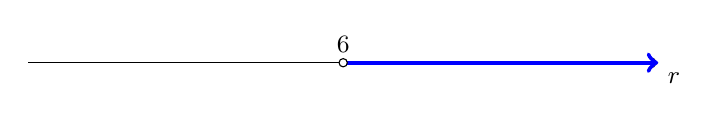
\begin{tikzpicture}[font=\small,x=10mm, y=5mm]

\draw[->] (0,0) -- (8,0) node [below right] () {$r$};
\node[above]  at (4,0) {6};
\begin{scope}[blue,ultra thick,->]
\draw (4,0) -- (8,0);
\end{scope}
\draw[fill=white] (4,0)circle (1.5pt);

\end{tikzpicture}
\end{center}
\end{enumeratea}
 \end{esempio}

 \begin{esempio}
 $\dfrac{(x+1)^{2}}{4}-\dfrac{2+3x}{2}>\dfrac{(x-1)^{2}}{4}.$
\end{esempio}
Il~$\mcm$ è~4 numero positivo, moltiplicando per~4 si ha
\[4\cdot\left[\frac{(x+1)^{2}}{4}-\frac{2+3x}{2}\right]>\frac{4\cdot{(x-1)^{2}}}{4}.\]
Semplificando:~$(x+1)^{2}-2\cdot (2+3x)>(x-1)^{2}$.

Eseguiamo i prodotti:~$x^{2}+2x+1-4-6x>x^{2}-2x+1$.

Eliminiamo dai due membri i termini uguali~$x^{2}$ e~1,
quindi trasportiamo a sinistra i monomi con l'incognita e a
destra i termini noti; infine sommiamo i monomi simili:

\[\cancel{{x^{2}}}+2x\cancel{+1}-4-6x>\cancel{{x^{2}}}-2x\cancel{+1}\quad \Rightarrow\quad~2x+2x-6x>+4
\quad\Rightarrow\quad -2x>4.\]

Il coefficiente dell'incognita è negativo, applicando
il terzo principio dividiamo ambo i membri per~$-2$ e cambiamo il verso
della disuguaglianza:
\[\frac{-2}{-2}x<\frac{4}{-2}\quad\Rightarrow\quad x<-2.\]

\begin{center}
 % (c) 2012 Dimitrios Vrettos - d.vrettos@gmail.com
\begin{tikzpicture}[font=\small,x=10mm, y=5mm]

\draw[->] (0,0) -- (8,0) node [below right] () {$r$};
\node[above]  at (4,0) {$-2$};
\begin{scope}[blue,thick]
\draw (0,0) -- (4,0);
\draw[fill=white] (4,0)circle (1.5pt);
\end{scope}

\end{tikzpicture}
\end{center}

 Quindi $\IS=\{x\in \insR\mid x<-2\}=(-\infty\text{,~}-2)$.


Alla stessa conclusione potevamo arrivare in altro modo. Giunti alla forma~$-2x>4$ trasportiamo a destra del
segno di disuguaglianza il monomio con l'incognita e a
sinistra il termine noto; ovviamente per il primo principio
questi termini spostandosi cambiano segno e otteniamo~$-4>2x$. Il coefficiente
dell'incognita è positivo dunque applichiamo il
secondo principio dividendo per~2,
abbiamo~$\dfrac{-4}{2}>\dfrac{2}{2}x\:\Rightarrow\: -2>x$, che letta da destra verso sinistra dice che i
valori da attribuire ad~$x$ per soddisfare la disequazione assegnata sono
tutti i numeri reali minori di~$-2$.

\vspace*{1.05ex}
\end{exrig}

Vediamo qualche esempio in cui scompare l'incognita.

\begin{exrig}

\begin{esempio}
$\dfrac{1}{2}\cdot (x+5)-x>\dfrac{1}{2}\cdot (3-x).$
\end{esempio}
Il~$\mcm$ è~2, positivo; moltiplichiamo ambo i membri per~2 e svolgiamo
i calcoli:

\[2\cdot \left[\frac{1}{2}(x+5)-x\right]>2\cdot
\left[\frac{1}{2}(3-x)\right]\quad\Rightarrow\quad x+5-2x>3-x\quad\Rightarrow\quad -x+5>3-x.\]

La forma canonica è~$0\cdot x>-2$ che si riduce alla disuguaglianza~$0>-2$
vera per qualunque~$x$ reale:~$\IS=\insR$.


\begin{esempio}
$(x+2)^2-4(x+1)<x^{2}-1.$
\end{esempio}
Svolgiamo i calcoli ed eliminiamo i monomi simili:
\[x^{2}+4x+4-4x-4<x^{2}-1\quad\Rightarrow\quad~0\cdot x<-1\]
che è la disuguaglianza~$0<-1$ falsa per qualunque~$x$ reale:~$\IS=\emptyset $.
\vspace*{1.05ex}
\end{exrig}

\ovalbox{\risolvii \ref{ese:20.9}, \ref{ese:20.10}, \ref{ese:20.11}, \ref{ese:20.12}, \ref{ese:20.13}, \ref{ese:20.14}, \ref{ese:20.15}}

\subsection{Problemi con le disequazioni}
 \begin{problema}[Tariffe telefoniche]
 Sto analizzando due proposte di compagnie telefoniche per poi stipulare
il contratto più conveniente per le mie esigenze. La compagnia
T\textsubscript{1} prevede una spesa fissa di~5 centesimi di scatto
alla risposta da sommare alla spesa di~1 centesimo per ogni minuto di
telefonata. La compagnia T\textsubscript{2} non prevede spesa per lo
scatto alla risposta, ma per ogni minuto di telefonata la spesa è di~2 centesimi.
Dopo quanti minuti di telefonata la seconda tariffa è
più conveniente della prima?
 \end{problema}

 \begin{soluzione}
 Indichiamo con~$x$ la durata in minuti di una telefonata e con
$s_{1}$ e~$s_{2}$ rispettivamente la spesa con
la prima e la seconda compagnia:

\[s_{1}=(5+1\cdot x)\text{ centesimi;}\quad s_{2}=(2\cdot x)\text{ centesimi.}\]

La~$s_2$ sarà più conveniente di~$s_1$ se~$s_{2} < s_{1} \:\Rightarrow\: 2\cdot x<5+x$.

Il problema è formalizzato con una disequazione
nell'incognita~$x$, di primo grado. Dobbiamo trovare l'$\IS$.

Risolvendo la disequazione si ottiene:
$2\cdot x-x<5\:\Rightarrow\: x<5\unit{min}$.

Conclusione: se le mie telefonate durano meno di~5~minuti allora mi
conviene il contratto con T\textsubscript{2}, altrimenti se faccio
telefonate più lunghe di~5~minuti mi conviene T\textsubscript{1}. Le
due tariffe sono uguali se la telefonata dura esattamente~5~minuti.
 \end{soluzione}


 \begin{problema}[L'abbonamento]
 Su un tragitto ferroviario, il biglietto costa~\officialeuro~$8,25$.
L'abbonamento mensile costa~\officialeuro~$67,30$. Qual è il
numero di viaggi che occorre effettuare in un mese perché
l'abbonamento risulti più conveniente?
 \end{problema}

 \begin{soluzione}
 Indichiamo con~$x$ il numero di viaggi. Il costo del biglietto di~$x$ viaggi
è~$8,25\cdot x$. L'abbonamento è più
conveniente quando~$8,25\cdot x>67,30$ da cui~$x>\dfrac{67,30}{8,25}$
e quindi~$x>8,16$. In conclusione se in un
mese si fanno fino a~8 viaggi conviene acquistare i biglietti singoli, da~9 viaggi in poi
conviene l'abbonamento.
 \end{soluzione}

 \ovalbox{\risolvii \ref{ese:20.16}, \ref{ese:20.17}, \ref{ese:20.18}, \ref{ese:20.19}, \ref{ese:20.20}, \ref{ese:20.21}, \ref{ese:20.22}, \ref{ese:20.23}, \ref{ese:20.24}, \ref{ese:20.25}, \ref{ese:20.26}}

\vspazio\ovalbox{\ref{ese:20.27}, \ref{ese:20.28}, \ref{ese:20.29}, \ref{ese:20.30}, \ref{ese:20.31}, \ref{ese:20.32}}

\section{Sistemi di disequazioni}
In alcune situazioni occorre risolvere contemporaneamente più
disequazioni. Vediamo alcuni problemi.

\begin{problema}
Il doppio di un numero reale positivo diminuito di~1 non supera la sua
metà aumentata di~2. Qual è il numero?
\end{problema}

\begin{soluzione}
 L'incognita del problema è il numero reale che indichiamo con~$x$. Di esso
sappiamo che deve essere positivo, quindi~$x>0$ e che deve verificare
la condizione
\[2x-1\le \frac{1}{2}x+2.\]
Le due disequazioni devono
verificarsi contemporaneamente.

Il problema può essere formalizzato con un \emph{sistema di disequazioni}:
\[\bigg \{%
\begin{array}{l}
 x>0\\
 2x-1\le\dfrac{1}{2}x+2
\end{array}.\]



\emph{Risolvere un sistema di disequazioni} significa trovare
l'insieme dei numeri reali che sono soluzioni comuni
alle disequazioni che lo compongono, cioè che le verificano tutte.

Se indichiamo con~$\IS_{1}$ e~$\IS_{2}$
rispettivamente gli insiemi soluzione della prima e della seconda
disequazione, l'insieme soluzione del sistema è dato
dall'intersezione
$\IS=\IS_{1}\cap\IS_{2}$.
\pagebreak

Risolviamo separatamente le due disequazioni e determiniamo gli
insiemi delle soluzioni.

\[d_1:\quad x>0\quad\Rightarrow\quad \IS_{1}=\{x\in\insR\mid x>0\}=(0\text{,~}+\infty)\text{,}\]
\[d_2:\quad 4x-2\le x+4\quad\Rightarrow\quad 3x\le~6\quad\Rightarrow\quad\IS_{2}=\{x\in \insR\mid x\le~2\}=(-\infty\text{,~}2].\]

Dobbiamo ora determinare~$\IS=\IS_{1}\cap\IS_{2}$.

Questa ricerca può essere facilitata rappresentando graficamente i due
intervalli in uno stesso schema. Disegniamo l'asse~$r$ dei
numeri reali e su esso indichiamo i numeri che entrano in gioco, lo~0
e il~2. Disegniamo una prima linea dove rappresentiamo con un tratto più
spesso~$\IS_{1}$, disegniamo una seconda linea dove
rappresentiamo con un tratto più spesso~$\IS_2$.

Su una terza linea rappresentiamo l'insieme degli
elementi comuni a~$\IS_{1}$ e~$\IS_{2}$, che
è appunto l'insieme delle soluzioni del sistema di
disequazioni.
\begin{center}
 % (c) 2012 Dimitrios Vrettos - d.vrettos@gmail.com
\begin{tikzpicture}[font=\small,x=10mm, y=10mm]

\draw[->] (0,0) -- (8,0) node [below right] () {$r$};

\foreach \x in {2,6}
\draw(\x,3pt)--(\x,-3pt);

\node[above]  at (2,0) {$0$};
\node[above]  at (6,0) {2};

\begin{scope}[dotted]
\draw (2,0) -- (2,-2);
\draw (6,0) -- (6,-2);
\draw (0,-.5) -- (2,-.5);
\draw (6,-.5) -- (8,-.5);
\end{scope}

\pattern[pattern= north east lines, pattern color=red] (2,-2) rectangle (6,-1.5);

\node[below] () at (4,-2) {$\IS$};

\begin{scope}[blue,thick]
\draw (2,-.5) -- (8,-.5);
\draw (0,-1) -- (6,-1);
\draw[fill=blue] (6,-1)circle (1.5pt);
\draw[fill=white] (2,-.5)circle (1.5pt);
\end{scope}

\end{tikzpicture}

\end{center}

Non ci rimane che descrivere
l'intervallo delle soluzioni in forma insiemistica:
\[\IS=\{x\in \insR\mid 0<x\le~2\}=(0\text{,~}2].\]

\end{soluzione}

\begin{problema}
 In un triangolo il lato maggiore misura~$13\unit{m}$ e gli altri due lati
differiscono tra di loro di~$2\unit{m}$. Come si deve scegliere il lato minore
affinché il perimetro non superi i~$100\unit{m}$?
\end{problema}

\emph{Dati}:~$\overline{AB}=13\unit{m}$, $\overline{BC}-\overline{AC}=2\unit{m}$.
Riferendoci alla figura, $AC$ è il lato minore; indichiamo con~$x$ la sua
misura.
\begin{center}
 % (c) 2012 Dimitrios Vrettos - d.vrettos@gmail.com
\begin{tikzpicture}[font=\small,x=10mm, y=10mm]

\draw (0,0) -- (2,3)--(6,0)--(0,0);

\node[left] at (0,0) {$A$};
\node[right] at (6,0) {$B$};
\node[above] at (2,3) {$C$};
\end{tikzpicture}
\end{center}

\emph{Obiettivo}: determinare~$x$ in modo che~$2p\le~100$.

\begin{soluzione}
 $\overline{AC}=x$; $\overline{BC}=2+x$; $\overline{AB}=13$ con $x>0$.

L'obiettivo, in linguaggio matematico, si scrive:~$x+(2+x)+13\le~100$.


Per la ``disuguaglianza triangolare''
si deve avere~$x+(2+x)>13$, altrimenti i tre lati non riescono a formare un triangolo.

Inoltre $\overline{AC}<\overline{AB}$ e $\overline{BC}<\overline{AB}$, altrimenti $AB$ non è più il lato maggiore.

Il problema è quindi formalizzato dal sistema:

\[\left\{%
\begin{array}{l}
x>0\\
x+(x+2)+13\le~100\\
x+(x+2)>13\\
x<13\\
x+2<13
\end{array}
\right.\]

Risolvendo ciascuna disequazione si ottiene:

{\longarray\[\left\{%
\begin{array}{l}
x>0\\
x\le\dfrac{85}{2}\\
x>\dfrac{11}{2}\\
x<13\\
x<11
\end{array}
\right.\]}

Determiniamo l'insieme soluzione aiutandoci con una
rappresentazione grafica (tenendo conto del fatto che $85/2 = 42,5$ e $11/2=5,5$).
\begin{center}
 % (c) 2012 Dimitrios Vrettos - d.vrettos@gmail.com
\begin{tikzpicture}[font=\small,x=10mm, y=10mm]

\draw[->] (-1.5,0) -- (8,0) node [below right] () {$r$};

\foreach \x in {0,1,2.5,3,7}{
\draw (\x,3pt)--(\x,-3pt);
\begin{scope}[dotted]
\draw (\x,0) -- (\x,-3.5);
\draw (-1.5,-.5) -- (0,-.5);
\draw (-1.5,-1) -- (1,-1);
\draw (7,-1.5) -- (8,-1.5);
\draw (3,-2) -- (8,-2);
\draw (2.5,-2.5) -- (8,-2.5);
\end{scope}}

\node[above]  at (0,0) {$0$};
\node[above]  at (1,0) {$\frac{11}{2}$};
\node[above]  at (7,0) {$\frac{85}{2}$};
\node[above]  at (3,0) {$13$};
\node[above]  at (2.5,0) {$11$};
\pattern[pattern= north east lines, pattern color=red] (1,-3.5) rectangle (2.5,-3);

\node[below] () at (1.75,-3.5) {$\IS$};

\begin{scope}[blue,thick]
\draw (0,-.5) -- (8,-.5);
\draw (1,-1) -- (8,-1);
\draw (-1.5,-1.5) -- (7,-1.5);
\draw (-1.5,-2) -- (3,-2);
\draw (-1.5,-2.5) -- (2.5,-2.5);

\draw[fill=white] (0,-.5)circle (1.5pt);
\draw[fill=white] (1,-1)circle (1.5pt);
\draw[fill=blue] (7,-1.5)circle (1.5pt);
\draw[fill=white] (3,-2)circle (1.5pt);
\draw[fill=white] (2.5,-2.5)circle (1.5pt);
\end{scope}

\end{tikzpicture}

\end{center}
Affinché il perimetro non superi~$100\unit{m}$ (e la figura sia sempre un triangolo con il lato maggiore di~$13\unit{m}$) la misura in metri del
lato minore deve essere un numero dell'insieme:
\[\IS=\left\{x\in \insR\mid \frac{11}{2}<x<11\right\} = \left(\frac{11}{2}\text{,~}11\right).\]
\end{soluzione}

Risolviamo delle disequazioni più articolate nel calcolo algebrico.

\begin{exrig}
 \begin{esempio}
Risolvere il seguente sistema di disequazioni
\longarray{
\[\left\{%
 \begin{array}{l}
  x>\dfrac{2x-11}{8}+\dfrac{19-2x}{4}\\
  \dfrac{1}{5}(x+1)>\dfrac{x}{3}-\dfrac{15+2x}{9}
  \end{array}
\right..\]}

Risolviamo separatamente le due disequazioni:

\[D_{1}:\quad 8x>2x-11+38-4x\Rightarrow~10x>27\Rightarrow x>\frac{27}{10}\rightarrow\IS_{1}=\left\{x\in\insR\mid x>\frac{27}{10}\right\}\text{,}\]
\[D_{2}:\quad 9x+9>15x-75-10x\Rightarrow~4x>-84\Rightarrow x>-21\rightarrow \IS_{2}=\left\{x\in\insR\mid x>-21\right\}.\]

Rappresentiamo graficamente le soluzioni e determiniamo~$\IS=\IS_{1}\cap \IS_{2}$:
\begin{center}
% (c) 2012 Dimitrios Vrettos - d.vrettos@gmail.com
\begin{tikzpicture}[font=\small,x=10mm, y=10mm]

\draw[->] (0,0) -- (8,0) node [below right] () {$r$};

\foreach \x in {2,6}{
\draw(\x,3pt)--(\x,-3pt);
\begin{scope}[dotted]
\draw (\x,0) -- (\x,-2);
\draw (0,-.5) -- (2,-.5);
\draw (0,-1) -- (6,-1);
\end{scope}}

\node[above]  at (2,0) {$-21$};
\node[above]  at (6,0) {$\frac{27}{10}$};
\pattern[pattern= north east lines, pattern color=red] (6,-1.5) rectangle (8,-2);

\node[below] () at (7,-2) {$\IS$};

\begin{scope}[blue,thick]
\draw (2,-.5) -- (8,-.5);
\draw (6,-1) -- (8,-1);

\draw[fill=white] (2,-.5)circle (1.5pt);
\draw[fill=white] (6,-1)circle (1.5pt);

\end{scope}

\end{tikzpicture}

\end{center}
\[\IS=\left\{x\in\insR\mid x>\frac{27}{10}\right\}.\]
 \end{esempio}

 \begin{esempio}
 Risolvere il seguente sistema di disequazioni
 \longarray{
 \[\left\{%
 \begin{array}{l}
  2\cdot (x+1)+(-2)^{2}\cdot x>3\cdot(2x-3)\\
  \dfrac{(x-3)^{2}}{4}-\dfrac{(2x-1)^{2}}{16}<\dfrac{35}{16}
 \end{array}
\right..\]}

Risolviamo separatamente le due disequazioni:

\[D_{1}:\quad 2x+2+4x>6x-9\Rightarrow~0x>-11\rightarrow\IS_{1}=\insR,\]
\[D_{2}:\quad 4x^{2}+36-24x-4x^{2}-1+4x-35<0\Rightarrow -20x<0\Rightarrow x>0\rightarrow\IS_{2}=\left\{x\in \insR\mid x>0\right\}.\]

Determiniamo~$\IS=\IS_{1}\cap \IS_{2}$.
\begin{center}
% (c) 2012 Dimitrios Vrettos - d.vrettos@gmail.com
\begin{tikzpicture}[font=\small,x=10mm, y=10mm]

\draw[->] (0,0) -- (8,0) node [below right] () {$r$};

\draw(4,3pt)--(4,-3pt);

\begin{scope}[dotted]
\draw (4,0) -- (4,-2);
\draw (0,-.5) -- (2,-.5);
\draw (0,-1) -- (4,-1);
\end{scope}

\node[above]  at (4,0) {$0$};
\pattern[pattern= north east lines, pattern color=red] (4,-1.5) rectangle (8,-2);

\node[below] () at (6,-2) {$\IS$};

\begin{scope}[blue,thick]
\draw (0,-.5) -- (8,-.5);
\draw (4,-1) -- (8,-1);

\draw[fill=white] (4,-1)circle (1.5pt);

\end{scope}

\end{tikzpicture}

\end{center}
 \[\IS=\left\{x\in \insR\mid x>0\right\}.\]
 \end{esempio}

 \begin{esempio}
 Risolvere il seguente sistema di disequazioni
\longarray{
\[\left\{%
 \begin{array}{l}
  (x-2)\cdot (x+3)\ge x+(x-1)\cdot (x+1)\\
  (x-1)^{3}\le x^{2}\cdot(x-3)+2\left(-{\dfrac{1}{2}}x+1\right)
 \end{array}
\right..\]}

Risolviamo separatamente le disequazioni:
\[D_{1}:\quad x^{2}-2x+3x-6>x+x^{2}-1\Rightarrow~0x\ge~5\rightarrow\IS_{1}=\emptyset.\]

Poiché la prima equazione non ha soluzioni, non avrà soluzioni
nemmeno il sistema. È superfluo quindi risolvere la
seconda disequazione. La risolviamo per esercizio.

\[D_{2}:\quad x^{3}-3x^{2}+3x-1\le x^{3}-3x^{2}-x+2\Rightarrow~4x\le~3\Rightarrow x\le\frac{3}{4}\rightarrow\IS_{2}=\left\{x\in \insR\mid x\le\frac{3}{4}\right\}.\]

\[\IS=\IS_{1}\cap \IS_{2}=\emptyset\cap\IS_{2}=\emptyset.\]
 \end{esempio}

 \begin{esempio}
 Risolvere il seguente sistema di disequazioni
\longarray{%
\[\left\{%
 \begin{array}{l}
  \dfrac{1}{3}\cdot\left(x-\dfrac{1}{2}\right)-\dfrac{1}{2}\cdot\left(x-\dfrac{1}{3}\right)\le\dfrac{1}{6}\\
  x+1\le\dfrac{2x-1}{3}+\dfrac{1-2x}{4}
 \end{array}
\right..\]}

Risolviamo separatamente le due disequazioni:

\[D_{1}:\quad \frac{1}{3}x-\frac{1}{2}x\le \frac{1}{6}\Rightarrow~2x-3x\le~1\Rightarrow x\ge -1\rightarrow \IS_{1}=\{x\in\insR\mid x\ge -1\}\text{,}\]
\[D_{2}:\quad 12x+12\le~8x-4+3-6x\Rightarrow~10x\le -13\Rightarrow x\le -{\frac{13}{10}}\rightarrow\IS_{2}=\left\{x\in\insR\mid x\le -{\frac{13}{10}}\right\}.\]

Rappresentiamo le soluzioni e determiniamo
$\IS=\IS_{1}\cap \IS_{2}$.
\begin{center}
% (c) 2012 Dimitrios Vrettos - d.vrettos@gmail.com
\begin{tikzpicture}[font=\small,x=10mm, y=10mm]

\draw[->] (0,0) -- (8,0) node [below right] () {$r$};

\foreach \x in {2,5}{
\draw(\x,3pt)--(\x,-3pt);
\begin{scope}[dotted]
\draw (\x,0) -- (\x,-1.5);
\draw (0,-.5) -- (5,-.5);
\draw (2,-1) -- (8,-1);
\end{scope}}

\node[above]  at (5,0) {$-1$};
\node[above]  at (2,0) {$-\frac{13}{10}$};

\begin{scope}[blue,thick]
\draw (5,-.5) -- (8,-.5);
\draw (0,-1) -- (2,-1);

\draw[fill=blue] (5,-.5)circle (1.5pt);
\draw[fill=blue] (2,-1)circle (1.5pt);

\end{scope}

\end{tikzpicture}
\end{center}

Il grafico mette in evidenza che i due insiemi soluzione non hanno
elementi in comune, pertanto~$\IS=\emptyset $.
 \end{esempio}
\end{exrig}

\ovalbox{\ref{ese:20.33}, \ref{ese:20.34}, \ref{ese:20.34}, \ref{ese:20.35}, \ref{ese:20.36}, \ref{ese:20.37}, \ref{ese:20.38}, \ref{ese:20.39}, \ref{ese:20.40}, \ref{ese:20.41}}

\section{Disequazioni polinomiali di grado superiore al primo}

\begin{problema}
\label{pro:20.1}
Determinare i valori di~$x$ che rendono il polinomio~$P=(3x-7)(2-x)$ positivo.
\end{problema}

Il problema chiede di determinare l'insieme delle
soluzioni della disequazione di secondo grado~$(3x-7)(2-x)>0$. La
disequazione si presenta nella forma di prodotto di due fattori di
primo grado e proprio la sua forma di prodotto ci faciliterà la
risposta al quesito.
\begin{wrapfloat}{figure}{r}{0pt}
 % (c) 2012 Dimitrios Vrettos - d.vrettos@gmail.com
\begin{tikzpicture}[font=\small,x=10mm, y=10mm]

\matrix (a)[matrix of nodes]{
$\times$& $+$ $-$\\
$+$& $+$ $-$\\
$-$& $-$ $+$\\
};

\begin{scope}[orange]
\draw (a-1-1.north east)--(a-3-1.south east);
\draw (a-1-1.south west)--(a-1-2.south east);
\end{scope}
\end{tikzpicture}
\end{wrapfloat}

Sappiamo che nell'insieme dei numeri relativi il segno
del prodotto di due fattori segue la regola dei segni visualizzata
dalla tabella a lato: ``il segno di un prodotto è
positivo se i due fattori sono concordi''. Questo
fatto si traduce nei due metodi risolutivi del problema proposto.

\begin{soluzione}
\textbf{Metodo I}: impostiamo due sistemi di disequazioni, formalizzando
l'osservazione precedente:

\[\left\{\begin{array}{l}
	 3x-7>0\\
	 2-x>0
	\end{array}
	 \right.\quad\vee\quad
 \left\{\begin{array}{l}
	 3x-7<0\\
	 2-x<0
	\end{array}
 \right..\]

 Risolvendo i due sistemi e unendo le loro soluzioni otteniamo
l'insieme delle soluzioni della disequazione
originaria:~$\IS=\IS_{1}\cup \IS_{2}$.

 \[\IS_{1}: \left\{\begin{array}{l}
		  3x-7>0\\
		  2-x>0
		 \end{array}
	  \right.
\Rightarrow\left\{\begin{array}{l}
		 x>\dfrac{7}{3}\\
		 x<2
		 \end{array}
	  \right.
\rightarrow \IS_{1}=\emptyset\text{,}\]
\[\IS_{2}: \left\{\begin{array}{l}
		 3x-7<0\\
		 2-x<0
		 \end{array}\right.
\Rightarrow\left\{\begin{array}{l}
		 x<\dfrac{7}{3}\\
		 x>2
		 \end{array}\right.
\rightarrow\IS_{2}=\left\{x\in\insR\mid 2<x<\dfrac{7}{3}\right\}.\]

Quindi~$\IS=\IS_{1}\cup\IS_{2}=\left\{x\in\insR\mid 2<x<\dfrac{7}{3}\right\}=\left(2\text{,~}\dfrac{7}{3}\right)$.

\textbf{Metodo~II}: Torniamo alla disequazione iniziale~$(3x-7)(2-x)>0$ e
applichiamo un altro metodo. Osserviamo che quando risolviamo la
disequazione~$3x-7>0$ determiniamo l'insieme
dei valori che attribuiti alla variabile rendono il polinomio~$P_1=3x-7$
positivo, precisamente sono i valori~$x>\frac{7}{3}$. Rappresentiamo
l'~$\IS$ con una semiretta in grassetto come in figura:
\begin{center}
% (c) 2012 Dimitrios Vrettos - d.vrettos@gmail.com
\begin{tikzpicture}[font=\small,x=10mm, y=10mm]

\draw[->] (0,0) -- (8,0) node [below right] () {$r$};

\draw(4,3pt)--(4,-3pt);

\node[above]  at (4,0) {$\frac{7}{3}$};

\begin{scope}[blue,thick,->]
\draw (4,0) -- (8,0);
\draw[fill=white] (4,0)circle (1.5pt);
\end{scope}

\end{tikzpicture}
\end{center}

In realtà, nel grafico sono contenute tutte le informazioni sul segno
del polinomio:

\begin{itemize*}
\item la semiretta in grassetto rappresenta i valori che rendono il polinomio $P_1$ positivo;
\item il valore~$x = \frac{7}{3}$ è quello che annulla il polinomio $P_1$;
\item la semiretta non in grassetto rappresenta i valori che rendono il polinomio $P_1$ negativo.
\end{itemize*}

\begin{center}
 % (c) 2012 Dimitrios Vrettos - d.vrettos@gmail.com
\begin{tikzpicture}[font=\small,x=10mm, y=10mm]

\draw[->] (0,0) -- (8,0) node [below right] () {$r$};
\draw[dotted] (4,0) -- (4,-.5);

\draw(4,3pt)--(4,-3pt);

\node[above]  at (4,0) {$\frac{7}{3}$};
\begin{scope}[below]
\node at (6,0) {$+$};
\node at (2,0) {$-$};
\end{scope}
\begin{scope}[blue,thick,->]
\draw (4,0) -- (8,0);
\draw[fill=white] (4,0)circle (1.5pt);
\end{scope}

\end{tikzpicture}
\end{center}
\end{soluzione}

\ovalbox{\risolvii \ref{ese:20.42}, \ref{ese:20.43}}
\pagebreak

\begin{exrig}
 \begin{esempio}
 $(3x-7)\cdot (2-x)>0.$

 La disequazione equivale a determinare i valori che, attribuiti alla
variabile~$x$, rendono positivo il polinomio~$P=(3x-7)\cdot (2-x)$.

Studiamo separatamente il segno dei due fattori:

\[F_{1}:\quad 3x-7>0\Rightarrow x>\frac{7}{3}\text{,}\quad
F_{2}:\quad 2-x>0\Rightarrow x<2.\]

Per risolvere la disequazione iniziale ci è di particolare aiuto un
grafico che sintetizzi la situazione.
\begin{center}
 % (c) 2012 Dimitrios Vrettos - d.vrettos@gmail.com
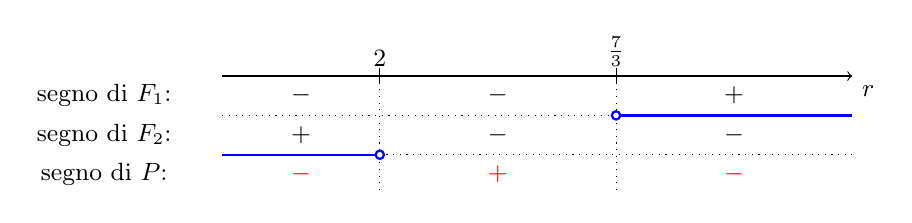
\begin{tikzpicture}[font=\small,x=10mm, y=10mm]

\draw[->] (0,0) -- (8,0) node [below right] () {$r$};

\foreach \x in {2,5}{
\draw(\x,3pt)--(\x,-3pt);
\begin{scope}[dotted]
\draw (\x,0) -- (\x,-1.5);
\draw (0,-.5) -- (5,-.5);
\draw (2,-1) -- (8,-1);
\end{scope}}

\node[above]  at (2,0) {$2$};
\node[above]  at (5,0) {$\frac{7}{3}$};

\begin{scope}[blue,thick]
\draw (5,-.5) -- (8,-.5);
\draw (0,-1) -- (2,-1);

\draw[fill=white] (5,-.5)circle (1.5pt);
\draw[fill=white] (2,-1)circle (1.5pt);
\end{scope}

\foreach \x in {-1.5}{
\node  at (\x,-.25) {segno di $F_1$:};
\node  at (\x,-.75) {segno di $F_2$:};
\node  at (\x,-1.25) {segno di $P$:};
}
\foreach \z in {1,3.5}{
\node  at (\z,-.25) {$-$};
}
\foreach \zi in {3.5, 6.5}{
\node  at (\zi,-.75) {$-$};
}

\node  at (6.5,-.25) {$+$};
\node  at (1,-.75) {$+$};

\begin{scope}[red]
\foreach \zii in {1, 6.5}{
\node  at (\zii,-1.25) {$-$};
}
\node  at (3.5,-1.25) {$+$};
\end{scope}
\end{tikzpicture}

\end{center}

Applicando poi la regola dei
segni otteniamo il segno del polinomio~$P=(3x-7)\cdot (2-x)$.

Ricordiamo che la disequazione che stiamo risolvendo~$(3x-7)\cdot(2-x)>0$
è verificata quando il polinomio~$P=(3x-7)\cdot (2-x)$ è
positivo, cioè nell'intervallo in cui abbiamo
ottenuto il segno ``$+$''. Possiamo
concludere~$\IS=\left\{x\in\insR\mid 2<x<\frac{7}{3}\right\}=(2\text{,~}\frac{7}{3})$.
 \end{esempio}

 \begin{esempio}
$(x-3)\cdot (2x-9)\cdot (4-5x)>0.$

Determiniamo il segno di ciascuno dei suoi tre fattori:

\[
F_{1}: x-3>0\:\Rightarrow\: x>3;\quad
F_{2}: 2x-9>0\:\Rightarrow\: x>\frac{9}{2};\quad
F_{3}: 4-5x>0\:\Rightarrow\: x<\frac{4}{5}.
\]

Costruiamo la tabella dei segni:
\begin{center}
 % (c) 2012 Dimitrios Vrettos - d.vrettos@gmail.com
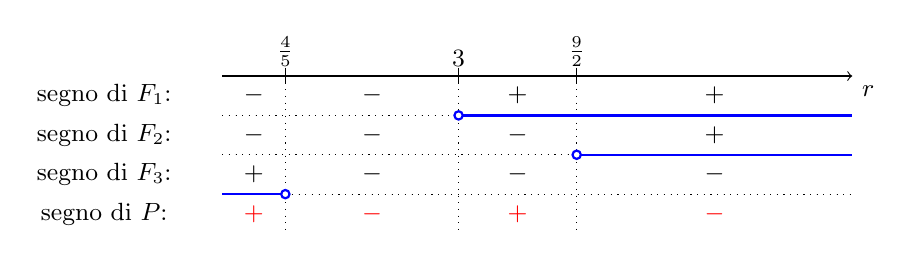
\begin{tikzpicture}[font=\small,x=10mm, y=10mm]

  \draw[->] (0,0) -- (8,0) node [below right] () {$r$};

  \foreach \x in {.8,3,4.5}{
    \draw(\x,3pt)--(\x,-3pt);

  \begin{scope}[dotted]
    \draw (\x,0) -- (\x,-2);
    \draw (0,-.5) -- (3,-.5);
    \draw (0,-1) -- (4.5,-1);
    \draw (.8,-1.5) -- (8,-1.5);
  \end{scope}}

  \node[above] at (.8,0) {$\frac{4}{5}$};
  \node[above]  at (3,0) {$3$};
  \node[above]  at (4.5,0) {$\frac{9}{2}$};

  \begin{scope}[blue,thick]
    \draw (3,-.5) -- (8,-.5);
    \draw (4.5,-1) -- (8,-1);
    \draw (0,-1.5) -- (.8,-1.5);

    \draw[fill=white] (3,-.5)circle (1.5pt);
    \draw[fill=white] (4.5,-1)circle (1.5pt);
    \draw[fill=white] (.8,-1.5)circle (1.5pt);
  \end{scope}

  \foreach \x in {-1.5}{
    \node  at (\x,-.25) {segno di $F_1$:};
    \node  at (\x,-.75) {segno di $F_2$:};
    \node  at (\x,-1.25) {segno di $F_3$:};
    \node  at (\x,-1.75) {segno di $P$:};
  }
  
  \foreach \z in {.4,1.9}
    \node  at (\z,-.25) {$-$};
  
  \foreach \zi in {.4,1.9, 3.75}
    \node  at (\zi,-.75) {$-$};

  \foreach \zii in {1.9, 3.75,6.25}
    \node  at (\zii,-1.25) {$-$};

  \foreach \ziii in {3.75,6.25}
    \node  at (\ziii,-.25) {$+$};

    \node  at (6.25,-.75) {$+$};
    \node  at (.4,-1.25) {$+$};

  \begin{scope}[red]
    \foreach \y in {-1.75}{
      \foreach \ziv in {.4,3.75}
	\node at (\ziv,\y) {$+$};
      \foreach \zv in {1.9,6.25}
	\node at (\zv,\y) {$-$};
      }
  \end{scope}
\end{tikzpicture}
\end{center}

La disequazione è verificata negli intervalli dove è presente il
segno ``$+$''.
\[\IS=\left\{x\in\insR\mid x<\frac{4}{5}\vee~3<x<\frac{9}{2}\right\}.\]
\end{esempio}

\begin{esempio}
 $4x^{3}+4x^{2}\le~1+x.$

La disequazione è di terzo grado. Trasportiamo al primo membro tutti i
monomi:
\[4x^{3}+4x^{2}-1-x\le~0.\]

Possiamo risolverla se riusciamo a scomporre in fattori di primo grado
il polinomio al primo membro:
\[4x^{3}+4x^{2}-1-x=4x^{2}(x+1)-(x+1)=(x+1)(4x^2-1)\:\Rightarrow\: (x+1)(2x-1)(2x+1)\le~0.\]

Studiamo ora il segno di ciascun fattore, tenendo conto che sono
richiesti anche i valori che annullano ogni singolo fattore (legge di
annullamento del prodotto):

\[ F_{1}:x+1\ge~0\:\Rightarrow\: x\ge -1;\quad F_{2}:2x-1\ge~0\:\Rightarrow\: x\ge \frac{1}{2};\quad F_{3}:2x+1\ge~0\:\Rightarrow\: x\ge -{\frac{1}{2}}.\]

Possiamo ora costruire la tabella dei segni.
Ricordiamo che la disequazione $P$ di partenza~$4x^{3}+4x^{2}\le~1+x$ è
verificata dove compare il segno~``$-$'':

\begin{center}
% (c) 2012 - 2013 Dimitrios Vrettos - d.vrettos@gmail.com
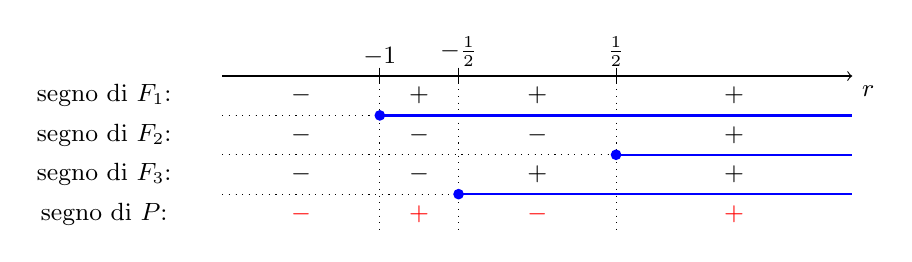
\begin{tikzpicture}[font=\small,x=10mm, y=10mm]

  \draw[->] (0,0) -- (8,0) node [below right] () {$r$};

  \foreach \x in {2,3,5}{
    \draw(\x,3pt)--(\x,-3pt);
    \begin{scope}[dotted]
      \draw (\x,0) -- (\x,-2);
      \draw (0,-.5) -- (2,-.5);
      \draw (0,-1) -- (5,-1);
      \draw (0,-1.5) -- (3,-1.5);
    \end{scope}}

  \node[above]  at (2,0) {$-1$};
  \node[above] at (3,0) {$-\frac{1}{2}$};
  \node[above]  at (5,0) {$\frac{1}{2}$};

  \begin{scope}[blue,thick]
    \draw (2,-.5) -- (8,-.5);
    \draw (5,-1) -- (8,-1);
    \draw (3,-1.5) -- (8,-1.5);

    \draw[fill=blue] (2,-.5)circle (1.5pt);
    \draw[fill=blue] (5,-1)circle (1.5pt);
    \draw[fill=blue] (3,-1.5)circle (1.5pt);
  \end{scope}

  \foreach \x in {-1.5}{
    \node  at (\x,-.25) {segno di $F_1$:};
    \node  at (\x,-.75) {segno di $F_2$:};
    \node  at (\x,-1.25) {segno di $F_3$:};
    \node  at (\x,-1.75) {segno di $P$:};}
  
  \foreach \z in {2.5,4,6.5}
    \node  at (\z,-.25) {$+$};
  
  \foreach \zi in {1,2.5, 4}
    \node  at (\zi,-.75) {$-$};
    
  \foreach \zii in {1,2.5}
    \node  at (\zii,-1.25) {$-$};
  

  \foreach \ziii in {4,6.5}
    \node  at (\ziii,-1.25) {$+$};

  \node  at (1,-.25) {$-$};
  \node  at (6.5,-.75) {$+$};


  \begin{scope}[red]
  \foreach \y in {-1.75}{
    \foreach \ziv in {2.5,6.5}
      \node at (\ziv,\y) {$+$};
    \foreach \zv in {1,4}
      \node at (\zv,\y) {$-$};
  }
  \end{scope}
\end{tikzpicture}

\end{center}
\[\IS=\left\{x\in \insR\mid x\le-1\text{ oppure }-\frac{1}{2}\le x\le\frac{1}{2}\right\}.\]
\end{esempio}
\end{exrig}

\begin{procedura}
 Determinare l'$\IS$ Di una disequazione polinomiale di grado
superiore al primo:

\begin{enumeratea}
 \item scrivere la disequazione nella forma~$P\leq0$, $P\geq~0$,
$P<0$, $P>0$;
\item scomporre in fattori irriducibili il polinomio $P$;
\item determinare il segno di ciascun fattore, ponendolo sempre maggiore
di zero, o maggiore uguale a zero a seconda della richiesta del
problema;
\item costruire la tabella dei segni, segnando con un punto ingrossato
gli zeri del polinomio;
\item determinare gli intervalli in cui il polinomio assume il segno
richiesto.
\end{enumeratea}
\end{procedura}

\ovalbox{\risolvii \ref{ese:20.44}, \ref{ese:20.45}, \ref{ese:20.46}, \ref{ese:20.47}, \ref{ese:20.48}, \ref{ese:20.49}, \ref{ese:20.50}, \ref{ese:20.51},
\ref{ese:20.52}, \ref{ese:20.53}}

\section{Disequazioni frazionarie}
Un'espressione contenente operazioni tra frazioni
algebriche ha come risultato una frazione algebrica. Con la condizione
di esistenza che il denominatore della frazione sia diverso da zero, la
ricerca del segno di una frazione algebrica viene effettuata con la
stessa procedura seguita per il prodotto di due o più fattori.

\begin{exrig}
 \begin{esempio}
 $P=\dfrac{3x-7}{2-x}\ge~0$.

 Poniamo innanzi tutto la~$\CE: 2-x\neq~0$
 cioè~$x\neq~2$ e procediamo studiando il segno del
numeratore $N$ e del denominatore $D$. Terremo conto della~$\CE$ ponendo il
denominatore $D$ semplicemente maggiore di zero e non maggiore uguale.
\[N\ge~0\:\Rightarrow\:~3x-7\ge~0\:\Rightarrow\: x\ge \frac{7}{3}\text{,}\]
\[D>0\:\Rightarrow\: 2-x>0\:\Rightarrow\: x<2.\]
\begin{center}
% (c) 2012 Dimitrios Vrettos - d.vrettos@gmail.com
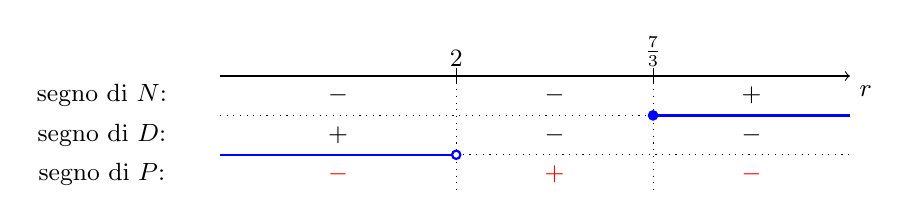
\begin{tikzpicture}[font=\small,x=10mm, y=10mm]

\draw[->] (0,0) -- (8,0) node [below right] () {$r$};

\foreach \x in {3,5.5}{
\draw(\x,3pt)--(\x,-3pt);
\begin{scope}[dotted]
\draw (\x,0) -- (\x,-1.5);
\draw (0,-.5) -- (5.5,-.5);
\draw (3,-1) -- (8,-1);
\end{scope}}

\node[above]  at (3,0) {$2$};
\node[above]  at (5.5,0) {$\frac{7}{3}$};

\begin{scope}[blue,thick]
\draw (5.5,-.5) -- (8,-.5);
\draw (3,-1) -- (0,-1);

\draw[fill=blue] (5.5,-.5)circle (1.5pt);
\draw[fill=white] (3,-1)circle (1.5pt);
\end{scope}

\foreach \x in {-1.5}{
\node  at (\x,-.25) {segno di $N$:};
\node  at (\x,-.75) {segno di $D$:};
\node  at (\x,-1.25) {segno di $P$:};
}
\foreach \z in {1.5,4.25}
\node  at (\z,-.25) {$-$};

\foreach \zi in {4.25,6.75}
\node  at (\zi,-.75) {$-$};

\node  at (6.75,-.25) {$+$};
\node  at (1.5,-.75) {$+$};

\begin{scope}[red]
\foreach \y in {-1.25}{
\foreach \ziv in {4.25}
	\node at (\ziv,\y) {$+$};
\foreach \zv in {1.5,6.75}
\node at (\zv,\y) {$-$};
}
\end{scope}
\end{tikzpicture}
\end{center}

Analogamente a quanto fatto per il prodotto, dalla tabella dei segni otteniamo
\[\IS=\left\{x\in \insR\mid 2<x\le \frac{7}{3}\right\}=\left(2\text{,~}\frac{7}{3}\right]\]
in cui vediamo già compresa la~$\CE$ che inizialmente avevamo posto.
 \end{esempio}
\end{exrig}

\begin{procedura}
 Procedura per determinare~$\IS$ di una disequazione frazionaria:

\begin{enumeratea}
\item applicare il primo principio e trasportare tutti i termini al primo membro;
 \item eseguire i calcoli dell'espressione al primo membro per arrivare a una disequazione nella forma:
 \subitem $\dfrac{N(x)}{D(x)}>0$ oppure~$\dfrac{N(x)}{D(x)}\ge~0$ oppure~$\dfrac{N(x)}{D(x)}<0$ oppure~$\dfrac{N(x)}{D(x)}\le~0$;
 \item studiare il segno del numeratore e del denominatore, ponendo~$N(x)>0$ (oppure~$N(x)\geq~0$ a secondo della richiesta) e~$D(x)>0$;
 \item costruire la tabella dei segni, segnando con un punto in grassetto gli zeri del numeratore;
 \item determinare gli intervalli in cui il polinomio assume il segno richiesto.
\end{enumeratea}
\end{procedura}

\begin{exrig}
 \begin{esempio}
 $\dfrac{x-1}{2x+2}+\dfrac{2x+1}{4x-2}>\dfrac{4x^{2}(2x+1)+1}{8x^{3}+8x^{2}-2x-2}.$

Trasportiamo tutti i termini al primo membro~$\dfrac{x-1}{2x+2}+\dfrac{2x+1}{4x-2}-\dfrac{4x^{2}(2x+1)+1}{8x^{3}+8x^{2}-2x-2}>0$.

Scomponiamo in fattori i denominatori, determiniamo il minimo comune
multiplo e sommiamo le frazioni per arrivare alla forma~$\frac{N(x)}{D(x)}>0$:

\begin{align}
&\frac{x-1}{2(x+1)}+\frac{2x+1}{2(2x-1)}-\frac{4x^{2}(2x+1)+1}{2(x+1)(2x-1)(2x+1)}>0 \notag\\
\Rightarrow & \frac{(x-1)(2x-1)(2x+1)+(2x+1)(2x+1)(x+1)-4x^{2}(2x+1)+1}{2(x+1)(2x-1)(2x+1)}>0 \notag\\
\Rightarrow & \frac{4x+1}{2(x+1)(2x-1)(2x+1)}>0. \label{eq:20.1}
\end{align}

Studiamo separatamente il segno di tutti i fattori che compaiono nella
frazione $F$, sia quelli al numeratore $N$ sia quelli al denominatore $D$ e
costruiamo la tabella dei segni:
 \[\begin{gathered}
 N>0\:\Rightarrow\: 4x+1>0\:\Rightarrow\: x>-{\frac{1}{4}}\text{,}\\
 D>0\:\Rightarrow\:\left\{\begin{array}{l}
			d_1:\: x+1>0\:\Rightarrow\: x>-1 \\
			d_2:\: 2x-1>0\:\Rightarrow\: x>\frac{1}{2}\\
			d_3:\: 2x+1>0\:\Rightarrow\: x>-{\frac{1}{2}}
		  \end{array}\right..
\end{gathered}\]
\begin{center}
% (c) 2012 Dimitrios Vrettos - d.vrettos@gmail.com
\begin{tikzpicture}[font=\small,x=10mm, y=10mm]

  \draw[->] (0,0) -- (8,0) node [below right] () {$r$};

  \foreach \x in {1.5,2.75,3.75,5.75}{
    \draw(\x,3pt)--(\x,-3pt);
    
    \begin{scope}[dotted]
      \draw (\x,0) -- (\x,-2.5);
      \draw (0,-.5) -- (3.75,-.5);
      \draw (0,-1) -- (1.5,-1);
      \draw (0,-1.5) -- (5.75,-1.5);
      \draw (0,-2) -- (2.75,-2);
    \end{scope}
  }

  \node[above]  at (1.5,0) {$-1$};
  \node[above] at (2.75,0) {$-\frac{1}{2}$};
  \node[above]  at (3.75,0) {$-\frac{1}{4}$};
  \node[above]  at (5.75,0) {$\frac{1}{2}$};

  \begin{scope}[blue,thick]
    \draw (3.75,-.5) -- (8,-.5);
    \draw (1.5,-1) -- (8,-1);
    \draw (5.75,-1.5) -- (8,-1.5);
    \draw (2.75,-2) -- (8,-2);

    \draw[fill=white] (3.75,-.5)circle (1.5pt);
    \draw[fill=white] (1.5,-1)circle (1.5pt);
    \draw[fill=white] (5.75,-1.5)circle (1.5pt);
    \draw[fill=white] (2.75,-2)circle (1.5pt);
  \end{scope}

  \foreach \x in {-1.5}{
    \node  at (\x,-.25) {segno di $N$:};
    \node(d1)  at (\x,-.75) {segno di $d_1$:};
    \node  at (\x,-1.25) {segno di $d_2$:};
    \node (d3) at (\x,-1.75) {segno di $d_3$:};
    \node  at (\x,-2.25) {segno di $F$ (\ref{eq:20.1}):};
    }

  \draw[decorate, decoration={brace, mirror}] let \p1=(d1.north west), \p2=(d3.south west) in(\p1 ) -- (\p2) node[midway, left=2pt] {$D:$};

  \foreach \z in {.75, 2.125,3.25}
    \node  at (\z,-.25) {$-$};

  \foreach \zi in {4.75, 6.875}
    \node  at (\zi,-.25) {$+$};

  \foreach \zii in {2.125,3.25,4.75, 6.875}
    \node  at (\zii,-.75) {$+$};

  \foreach \ziii in {.75,2.125,3.25,4.75}
    \node  at (\ziii,-1.25) {$-$};

  \foreach \ziv in {.75,2.125}
    \node at (\ziv,-1.75) {$-$};

  \foreach \zv in {3.25,4.75, 6.875}
    \node at (\zv,-1.75) {$+$};

  \node  at (.75,-.75) {$-$};
  \node  at (6.875,-1.25) {$+$};

  \begin{scope}[red]
    \foreach \y in {-2.25}{
      \foreach \ziv in {.75,3.25,6.875}
	\node at (\ziv,\y) {$+$};
      \foreach \zv in {2.125,4.75}
	\node at (\zv,\y) {$-$};
    }
  \end{scope}
\end{tikzpicture}

\end{center}
Non abbiamo posto le~$\CE$ in quanto già rispettate dalle disequazioni
del denominatore.
Prendiamo gli intervalli in cui il segno della frazione $F$ è positivo,
come richiesto dalla disequazione~\ref{eq:20.1}:
 \[\IS=\left\{x\in \insR\mid x<-1\vee -{\frac{1}{2}}<x<-{\frac{1}{4}}\vee x>\frac{1}{2}\right\}.\]
\end{esempio}

 \begin{esempio}
$\dfrac{x}{2}-\dfrac{2}{3}\cdot {\dfrac{2x-3}{x-1}}+\dfrac{10x-3}{6x-6}\le\dfrac{3}{2}\cdot {\dfrac{x^{2}+2}{3x-2}}+\dfrac{1}{3(x-1)(3x-2)}.$

Trasportiamo tutti i termini al primo membro:
\[\frac{x}{2}-\frac{2}{3}\cdot\frac{2x-3}{x-1}+\frac{10x-3}{6x-6}-\frac{3}{2}\cdot\frac{x^{2}+2}{3x-2}-\frac{1}{3(x-1)(3x-2)}\le~0.\]

Eseguiamo le operazioni per semplificare la frazione e ridurla alla
forma~$\frac{N(x)}{D(x)}\le~0$:

\begin{align}
  &\frac{x}{2}-\frac{4x-6}{3(x-1)}+\frac{10x-3}{6(x-1)}-\frac{3x^{2}+6}{2(3x-2)}-\frac{1}{3(x-1)(3x-2)}\le~0\notag\\
  \Rightarrow &\frac{3x(x-1)(3x-2)-2(4x-6)(3x-2)+(10x-3)(3x-2)-3(3x^{2}+6)(x-1)-2}{6(x-1)(3x-2)}\le~0\notag\\
  \Rightarrow &\frac{11x-2}{6(x-1)(3x-2)}\le~0. \label{eq:20.2}
\end{align}

Studiamo il segno di $F$, ovvero del suo numeratore $N$ e dei fattori del suo denominatore $D$:
 \[\begin{gathered}N\ge~0\:\Rightarrow\: 11x-2\ge 0\:\Rightarrow\: x\ge\frac{2}{11}\text{,}\\
		  D>0\:\Rightarrow\:\left\{\begin{array}{l}
			d_{1}>0\:\Rightarrow\: x-1>0\:\Rightarrow\: x>1\\
			d_{2}>0\:\Rightarrow\: 3x-2>0\:\Rightarrow\: x>\dfrac{2}{3}
			\end{array}\right.. \end{gathered}\]
\begin{center}
% (c) 2012 Dimitrios Vrettos - d.vrettos@gmail.com
\begin{tikzpicture}[font=\small,x=10mm, y=10mm]

\draw[->] (0,0) -- (8,0) node [below right] () {$r$};

\foreach \x in {1,3.72,5.56}{
\draw(\x,3pt)--(\x,-3pt);
\begin{scope}[dotted]
\draw (\x,0) -- (\x,-2);
\draw (0,-.5) -- (1,-.5);
\draw (0,-1) -- (5.56,-1);
\draw (0,-1.5) -- (3.72,-1.5);

\end{scope}}


\node[above] at (1,0) {$\frac{2}{11}$};
\node[above]  at (3.72,0) {$\frac{2}{3}$};
\node[above]  at (5.56,0) {$1$};

\begin{scope}[blue,thick]
\draw (1,-.5) -- (8,-.5);
\draw (5.56,-1) -- (8,-1);
\draw (3.72,-1.5) -- (8,-1.5);

\draw[fill=blue] (1,-.5)circle (1.5pt);
\draw[fill=white] (5.56,-1)circle (1.5pt);
\draw[fill=white] (3.72,-1.5)circle (1.5pt);
\end{scope}

\foreach \x in {-1.5}{
\node  at (\x,-.25) {segno di $N$:};
\node(d1)  at (\x,-.75) {segno di $d_1$:};
\node (d2) at (\x,-1.25) {segno di $d_2$:};
\node (d3) at (\x,-1.75) {segno di $F$ (\ref{eq:20.2}):};
}

 \draw[decorate, decoration={brace, mirror}]  let \p1=(d1.north west), \p2=(d2.south west) in(\p1 ) -- (\p2) node[midway, left=2pt] {$D:$};

\foreach \z in {2.36,4.64,6.78}
\node  at (\z,-.25) {$+$};

 \foreach \zi in {.5,2.36,4.64}
 \node  at (\zi,-.75) {$-$};

\foreach \zii in {.5,2.36}
 \node  at (\zii,-1.25) {$-$};

 \foreach \ziii in {4.64,6.78}
\node  at (\ziii,-1.25) {$+$};

\node  at (.5,-.25) {$-$};
\node  at (6.78,-.75) {$+$};

\begin{scope}[red]
\foreach \y in {-1.75}{
\foreach \ziv in {.5,4.64}
	\node at (\ziv,\y) {$-$};
\foreach \zv in {2.36,6.78}
\node at (\zv,\y) {$+$};
}
\end{scope}
\end{tikzpicture}

\end{center}
\pagebreak
Non abbiamo posto le~$\CE$ in quanto già rispettate dalle disequazioni
del denominatore. Prendiamo gli intervalli in cui il segno della frazione $F$ è positivo o
nullo, come dalla disequazione~\ref{eq:20.2}:
\[\IS=\left\{x\in \insR\mid x\le\frac{2}{11}\vee \frac{2}{3}<x<1\right\}.\]
 \end{esempio}
\end{exrig}
\ovalbox{\risolvii \ref{ese:20.54}, \ref{ese:20.55}, \ref{ese:20.56}, \ref{ese:20.57}, \ref{ese:20.58}, \ref{ese:20.59}, \ref{ese:20.60}, \ref{ese:20.61}, \ref{ese:20.62}, \ref{ese:20.63}}

\vspazio\ovalbox{\ref{ese:20.64}, \ref{ese:20.65}, \ref{ese:20.66}, \ref{ese:20.67}, \ref{ese:20.68}, \ref{ese:20.69}}
\newpage
% (c) 2012-2013 Claudio Carboncini - claudio.carboncini@gmail.com
% (c) 2012-2014 Dimitrios Vrettos - d.vrettos@gmail.com

\section{Esercizi}

\subsection{Esercizi dei singoli paragrafi}

\subsubsection*{\thechapter.1 - Equazioni di grado superiore al primo riducibili al primo grado}

\begin{esercizio}[\Ast]
\label{ese:20.1}
Risolvere le seguenti equazioni riconducendole a equazioni di primo grado.
\begin{multicols}{2}
\begin{enumeratea}
 \item $x^{2}+2x=0$;
 \item $x^{2}+2x-9x-18=0$;
 \item $2x^{2}-2x-4=0$;
 \item $4x^{2}+16x+16=0$.
\end{enumeratea}
\end{multicols}
\end{esercizio}

\begin{esercizio}[\Ast]
\label{ese:20.2}
Risolvere le seguenti equazioni riconducendole a equazioni di primo grado.
\begin{multicols}{2}
\begin{enumeratea}
 \item $x^{2}-3x-10=0$;
 \item $x^{2}+4x-12=0$;
 \item $3x^{2}-6x-9=0$;
 \item $x^{2}+5x-14=0$.
\end{enumeratea}
\end{multicols}
\end{esercizio}

\begin{esercizio}[\Ast]
\label{ese:20.3}
Risolvere le seguenti equazioni riconducendole a equazioni di primo grado.
\begin{multicols}{2}
\begin{enumeratea}
 \item $-3x^{2}-9x+30=0$;
 \item $-{\dfrac{3}{2}}x^{2}+\dfrac{3}{2}x+63=0$;
 \item $7x^{2}+14x-168=0$;
 \item $\dfrac{7}{2}x^{2}+7x-168=0$.
\end{enumeratea}
\end{multicols}
\end{esercizio}

\begin{esercizio}[\Ast]
\label{ese:20.4}
Risolvere le seguenti equazioni riconducendole a equazioni di primo grado.
\begin{multicols}{2}
\begin{enumeratea}
 \item $x^{4}-16x^{2}=0$;
 \item $2x^{3}+2x^{2}-20x+16=0$;
 \item $-2x^{3}+6x+4=0$;
 \item $-x^{6}+7x^{5}-10x^{4}=0$.
\end{enumeratea}
\end{multicols}
\end{esercizio}

\begin{esercizio}[\Ast]
\label{ese:20.5}
Risolvere le seguenti equazioni riconducendole a equazioni di primo grado.
\begin{multicols}{2}
\begin{enumeratea}
 \item $x^{3}-3x^{2}-13x+15=0$;
 \item $x^{2}+10x-24=0$;
 \item $2x^{3}-2x^{2}-24x=0$;
 \item $x^{4}-5x^{2}+4=0$.
\end{enumeratea}
\end{multicols}
\end{esercizio}

\begin{esercizio}[\Ast]
\label{ese:20.6}
Risolvere le seguenti equazioni riconducendole a equazioni di primo grado.
\begin{multicols}{2}
\begin{enumeratea}
 \item $-x^{3}-5x^{2}-x-5=0$;
 \item $\dfrac{3}{4}x^{3}-\dfrac{3}{4}x=0$;
 \item $-4x^{4}-28x^{3}+32x^{2}=0$;
 \item $-{\dfrac{6}{5}}x^{3}-\dfrac{6}{5}x^{2}+\dfrac{54}{5}x+\dfrac{54}{5}=0$.
\end{enumeratea}
\end{multicols}
\end{esercizio}

\begin{esercizio}[\Ast]
\label{ese:20.7}
Risolvere le seguenti equazioni riconducendole a equazioni di primo grado.
\begin{multicols}{2}
\begin{enumeratea}
 \item $-4x^{3}+20x^{2}+164x-180=0$;
 \item $5x^{3}+5x^{2}-80x-80=0$;
 \item $-3x^{3}+18x^{2}+3x-18=0$;
 \item $4x^{3}+8x^{2}-16x-32=0$.
\end{enumeratea}
\end{multicols}
\end{esercizio}

\begin{esercizio}[\Ast]
\label{ese:20.8}
Risolvere le seguenti equazioni riconducendole a equazioni di primo grado.
\begin{multicols}{2}
\begin{enumeratea}
 \item $x^{3}+11x^{2}+26x+16=0$;
 \item $2x^{3}+6x^{2}-32x-96=0$;
 \item $2x^{3}+16x^{2}-2x-16=0$;
 \item $-2x^{3}+14x^{2}-8x+56=0$.
\end{enumeratea}
\end{multicols}
\end{esercizio}
%\newpage
\begin{esercizio}[\Ast]
\label{ese:20.9}
Risolvere le seguenti equazioni riconducendole a equazioni di primo grado.
\begin{multicols}{2}
\begin{enumeratea}
 \item $2x^{3}+12x^{2}+18x+108=0$;
 \item $x^{4}-10x^{3}+35x^{2}-50x+24=0$;
 \item $-2x^{3}-12x^{2}+18x+28=0$;
 \item $-5x^{4}+125x^{2}+10x^{3}-10x-120=0$.
\end{enumeratea}
\end{multicols}
\end{esercizio}

\begin{esercizio}[\Ast]
\label{ese:20.10}
Risolvere le seguenti equazioni riconducendole a equazioni di primo grado.
\begin{multicols}{2}
\begin{enumeratea}
 \item $\dfrac{7}{6}x^{4}-\dfrac{161}{6}x^{2}-21x+\dfrac{140}{3}=0$;
 \item $(x^{2}-6x+8)(x^{5}-3x^{4}+2x^{3})=0$;
 \item $\left(25-4x^{2}\right)^{4}\left(3x-2\right)^{2}=0$;
 \item $(x-4)^{3}\left(2x^{3}-4x^{2}-8x+16\right)^{9}=0$.
\end{enumeratea}
\end{multicols}
\end{esercizio}

\begin{esercizio}[\Ast]
\label{ese:20.11}
Risolvere le seguenti equazioni riconducendole a equazioni di primo grado.
\begin{multicols}{2}
\begin{enumeratea}
 \item $(x^{3}-x)(x^{5}-9x^{3})(x^{2}+25)=0$;
 \item $x^{5}+3x^{4}-11x^{3}-27x^{2}+10x+24=0$;
 \item $2x^{2}-x-1=0$;
 \item $3x^{2}+5x-2=0$.
\end{enumeratea}
\end{multicols}
\end{esercizio}

\begin{esercizio}[\Ast]
\label{ese:20.12}
Risolvere le seguenti equazioni riconducendole a equazioni di primo grado.
\begin{multicols}{2}
\begin{enumeratea}
 \item $6x^{2}+x-2=0$;
 \item $2x^{3}-x^{2}-2x+1=0$;
 \item $3x^{3}-x^{2}-8x-4=0$;
 \item $8x^{3}+6x^{2}-5x-3=0$.
\end{enumeratea}
\end{multicols}
\end{esercizio}

\begin{esercizio}[\Ast]
\label{ese:20.13}
Risolvere le seguenti equazioni riconducendole a equazioni di primo grado.
\begin{multicols}{2}
\begin{enumeratea}
 \item $6x^{3}+x^{2}-10x+3=0$;
 \item $4x^{4}-8x^{3}-13x^{2}+2x+3=0$;
 \item $8x^{4}-10x^{3}-29x^{2}+40x-12=0$;
 \item $-12x^{3}+68x^{2}-41x+5=0$.
\end{enumeratea}
\end{multicols}
\end{esercizio}

\begin{esercizio}[\Ast]
\label{ese:20.14}
Risolvere la seguente equazione riconducendola a una equazione di primo grado.

$(x^{4}+3x^{3}-3x^{2}-11x-6)(4x^{6}-216x^{3}+2916)=0$;
\end{esercizio}

\subsubsection*{\thechapter.2 - Equazioni numeriche frazionarie}

\begin{esercizio}[\Ast]
\label{ese:20.15}
Risolvi le seguenti equazioni frazionarie.
\begin{multicols}{2}
\begin{enumeratea}
 \item $\dfrac{2}{x+1}=\dfrac{1}{x+2}$;
 \item $\dfrac{1}{x-1}=2$;
 \item $1-\dfrac{1}{x+1}=0$;
 \item $\dfrac{2x-4}{x-2}=0$.
\end{enumeratea}
\end{multicols}
\end{esercizio}

\begin{esercizio}[\Ast]
\label{ese:20.16}
Risolvi le seguenti equazioni frazionarie.
\begin{multicols}{2}
\begin{enumeratea}
 \item $\dfrac{x}{x+1}-\dfrac{1}{x-1}=1$;
 \item $\dfrac{1}{x-3}=\dfrac{x}{3-x}$;
 \item $\dfrac{x-1}{x^{2}-4}=-{\dfrac{5}{x+2}}$;
 \item $\dfrac{3}{x+1}=\dfrac{2}{x+1}$.
\end{enumeratea}
\end{multicols}
\end{esercizio}
%\newpage
\begin{esercizio}[\Ast]
\label{ese:20.17}
Risolvi le seguenti equazioni frazionarie.
\begin{multicols}{2}
\begin{enumeratea}
 \item $\dfrac{1}{3-x}-\dfrac{4}{2x-6}=0$;
 \item $\dfrac{x^{2}-1}{x-1}-1=2x+1$;
 \item $\dfrac{x}{x^{2}-4}=\dfrac{1}{x+2}$;
 \item $\dfrac{1}{x}-\dfrac{3}{x^{2}}=\dfrac{2-2x}{x^{3}}$.
\end{enumeratea}
\end{multicols}
\end{esercizio}

\begin{esercizio}[\Ast]
\label{ese:20.18}
Risolvi le seguenti equazioni frazionarie.
\begin{multicols}{2}
\begin{enumeratea}
 \item $\dfrac{x-2}{x-1}=\dfrac{x-1}{x-2}$;
 \item $\dfrac{x+3}{x+1}=x+3$;
 \item $\dfrac{3x+1}{3x^{2}+x}=1$;
 \item $\dfrac{6+x}{x-3}=\dfrac{x^{2}}{x-3}$.
\end{enumeratea}
\end{multicols}
\end{esercizio}

\begin{esercizio}[\Ast]
\label{ese:20.19}
Risolvi le seguenti equazioni frazionarie.
\begin{multicols}{2}
\begin{enumeratea}
 \item $\dfrac{1}{x-2}+\dfrac{2}{x+1}=\dfrac{3}{x^{2}-x-2}$;
 \item $\dfrac{5}{x-2}-\dfrac{6}{x+1}=\dfrac{3x-1}{x^{2}-x-2}$;
 \item $\dfrac{1}{1-x}-\dfrac{x}{x-1}=0$;
 \item $\dfrac{x+1}{x-1}-\dfrac{x}{1+x}=0$.
\end{enumeratea}
\end{multicols}
\end{esercizio}

\begin{esercizio}[\Ast]
\label{ese:20.20}
Risolvi le seguenti equazioni frazionarie.
\begin{multicols}{2}
\begin{enumeratea}
 \item $\dfrac{2x+1}{2x-1}+\dfrac{4x^{2}+1}{4x^{2}-1}=2$;
 \item $\dfrac{1}{x-1}+\dfrac{2}{x}+\dfrac{1}{x^{2}-x}=0$;
 \item $\dfrac{x-1}{x^{2}-2x+1}=\dfrac{2}{2-2x}$;
 \item $4-x^{2}=\dfrac{x^{2}+5x+6}{x+2}-1$.
\end{enumeratea}
\end{multicols}
\end{esercizio}

\begin{esercizio}[\Ast]
\label{ese:20.21}
Risolvi le seguenti equazioni frazionarie.
\begin{multicols}{2}
\begin{enumeratea}
 \item $\dfrac{5}{5x+1}+\dfrac{2}{2x-1}=\dfrac{1}{1-2x}$;
 \item $\dfrac{1}{x-2}+\dfrac{2}{x+1}=\dfrac{3}{x^{2}-x-2}$;
 \item $\dfrac{30}{x^{2}-25}+\dfrac{3}{5-x}=0$;
 \item $1+\dfrac{x-1}{x+1}=\dfrac{1}{x-2}+\dfrac{1-x^{2}}{x^{2}-x-2}$.
\end{enumeratea}
\end{multicols}
\end{esercizio}

\begin{esercizio}[\Ast]
\label{ese:20.22}
Risolvi le seguenti equazioni frazionarie.
\begin{multicols}{2}
\begin{enumeratea}
 \item $-{\dfrac{3x}{6-2x}}+\dfrac{5x}{10-5x}=\dfrac{1-x}{4-2x}$;
 \item $\dfrac{18x^{2}-9x-45}{4-36x^{2}}-\dfrac{6x+1}{9x-3}+\dfrac{21x-1}{18x+6}=0$;
 \item $\dfrac{1}{x+3}-\dfrac{1}{2-x}=\dfrac{x+3}{x^{2}+x-6}$;
 \item $\dfrac{1+2x}{1-2x}+\dfrac{1-2x}{1+2x}=\dfrac{6-8x^{2}}{1-4x^{2}}$.
\end{enumeratea}
\end{multicols}
\end{esercizio}

\begin{esercizio}[\Ast]
\label{ese:20.23}
Risolvi le seguenti equazioni frazionarie.
\begin{multicols}{2}
\begin{enumeratea}
 \item $\dfrac{3x}{x-2}+\dfrac{6x}{x^{2}-4x+4}=\dfrac{3x^{2}}{(x-2)^{2}}$;
 \item $(4x+6)\left(\dfrac{4}{x+1}-\dfrac{1}{x-1}\right)=0$;
 \item $\dfrac{5x}{3x^{2}-18x+15}-\dfrac{2}{3x-3}=\dfrac{5}{18x-90}$;
 \item $(x-4)(x+3)=\dfrac{(x-4)(x+3)}{x-2}$.
\end{enumeratea}
\end{multicols}
\end{esercizio}
%\newpage
\begin{esercizio}[\Ast]
\label{ese:20.24}
Risolvi le seguenti equazioni frazionarie.
\begin{multicols}{2}
\begin{enumeratea}
 \item $\dfrac{1}{3x+2}-\dfrac{3}{2-x}=\dfrac{10x+4}{3x^{2}-4x-4}$;
 \item $\dfrac{2x+1}{x+3}+\dfrac{1}{x-4}=\dfrac{4x-9}{x^{2}-x-12}$;
 \item $\dfrac{1}{x-1}-\dfrac{1}{x}=\dfrac{(x+1)^{2}}{2(x^{2}-1)}+1$;
 \item $\dfrac{x^{2}-1}{x+1}-\dfrac{1}{x+2}=\dfrac{x+1}{x+2}-x$.
\end{enumeratea}
\end{multicols}
\end{esercizio}

\begin{esercizio}[\Ast]
\label{ese:20.25}
Risolvi le seguenti equazioni frazionarie.
\begin{multicols}{2}
\begin{enumeratea}
 \item $\dfrac{1}{x+3}-\dfrac{2}{x+2}=\dfrac{3x-6}{x^{2}+5x+6}$;
 \item $\dfrac{2x-3}{x+2}+\dfrac{1}{x-4}=\dfrac{2}{x^{2}-2x-8}$;
 \item $\dfrac{x-1}{x+2}-\dfrac{x+2}{x-1}=\dfrac{1}{x^{2}+x-2}$;
 \item $\dfrac{3}{x-1}+\dfrac{1}{x+1}=\dfrac{12-x}{x^{2}-1}$.
\end{enumeratea}
\end{multicols}
\end{esercizio}

\begin{esercizio}[\Ast]
\label{ese:20.26}
Risolvi le seguenti equazioni frazionarie.
\begin{multicols}{2}
\begin{enumeratea}
 \item $\dfrac{1}{2} \left(x-\dfrac{1}{x}\right)-2\left(1-\dfrac{1}{x}\right)=\dfrac{x^{2}-1}{x}$;
 \item $\left(40-10x^{2}\right)^{3} \left(\dfrac{3x-1}{x+2}-\dfrac{3x}{x+1}\right)=0$;
 \item $\dfrac{x}{2x+1}+\dfrac{x+1}{2(x+2)}=\dfrac{x-1}{2x^{2}+5x+2}$;
 \item $\dfrac{3x+1}{x^{2}-9}+\dfrac{2}{3x^{2}-9x}=\dfrac{3}{x+3}$.
\end{enumeratea}
\end{multicols}
\end{esercizio}

\begin{esercizio}[\Ast]
\label{ese:20.27}
Risolvi le seguenti equazioni frazionarie.
\begin{multicols}{2}
\begin{enumeratea}
 \item $\dfrac{3(2x-3)}{x^{3}+27}+\dfrac{1}{x+3}=\dfrac{x}{x^{2}-3x+9}$;
 \item $\dfrac{1}{x^{2}-3x+2}+\dfrac{2}{x-1}=0$;
 \item $\dfrac{2x-1}{3x^{2}-75}-\dfrac{3-x}{x+5}+\dfrac{x-3}{10-2x}=\dfrac{7}{25-x^{2}}$;
 \item $\dfrac{x+2}{(x-3)^{2}}-\dfrac{1}{x-3}=\dfrac{4}{9-3x}$.
\end{enumeratea}
\end{multicols}
\end{esercizio}

\begin{esercizio}[\Ast]
\label{ese:20.28}
Risolvi le seguenti equazioni frazionarie.
\begin{enumeratea}
 \item $\left(\dfrac{1}{x+5}-\dfrac{1}{5}\right):\left(\dfrac{1}{x-5}+\dfrac{1}{5}\right)+\dfrac{x^{2}}{x^{2}-5x}=0$;
 \item $\dfrac{1+2x}{x^{2}+2x}+\dfrac{x^{3}-6x+1}{x^{2}-4}=\dfrac{x^{2}-2x}{x-2}+\dfrac{1}{x^{2}-2x}$.
 \item $\left(1-\dfrac{1}{2}x\right):\left(1+\dfrac{1}{2}x\right)=\dfrac{2x+1}{6x+3}-\dfrac{1}{2}x+\dfrac{x^{2}}{2x+4}$;
 \item $\dfrac{3x-1}{1-2x}+\dfrac{x}{2x-1}-\dfrac{x^{3}-8}{x^{2}-4}:\dfrac{x^{2}+2x+4}{x^{2}+2x+1}=\dfrac{2-3x}{2x-6}\cdot {\dfrac{x^{2}-9}{4-9x^{2}}}-\dfrac{6x+7}{6}$;
 \item $\dfrac{2x}{6x-3}+\dfrac{x}{4-8x}+\left(\dfrac{1}{2x+1}-\dfrac{1}{2x-1}\right)\cdot {\dfrac{2x\left(x^{2}-1\right)}{8x^{2}-4x}}=\dfrac{x^{2}(5x-3)}{3(2x+1)(2x-1)^{2}}$;
 \item $\dfrac{3x^{2}-2x+3}{x^{2}-3x}+\dfrac{x+2}{3-x}=\left(\dfrac{x+1}{x}-1\right)\left(\dfrac{x^{2}}{x^{3}-27}+\dfrac{x}{x-3}\right):\dfrac{3x}{3x^{3}-81}+\dfrac{x^{2}-x+2}{3-x}$.
\end{enumeratea}
\end{esercizio}

\begin{esercizio}
\label{ese:20.29}
$\left(2x-4x^{2}+7\right)^{6}=-{\dfrac{1}{\left(x^{2}-5x+7\right)^{4}}}$. Osservando i due membri dell'equazione, senza svolgere i calcoli, puoi subito affermare che non esiste alcun numero reale che rende
vera l'uguaglianza?
\end{esercizio}

\begin{esercizio}[\Ast]
\label{ese:20.30}
Quale numero occorre aggiungere a numeratore e denominatore della frazione tre settimi perchè essa raddoppi di valore?
\end{esercizio}

\begin{esercizio}[\Ast]
\label{ese:20.31}
Quale numero occorre aggiungere a numeratore e denominatore della frazione due settimi perchè essa triplichi di valore?
\end{esercizio}

\begin{esercizio}
\label{ese:20.32}
Due amici A e B partono con le loro automobili nello stesso istante da due località diverse; A fa un viaggio di
$100\unit{km}$ a una certa velocità, B fa un viaggio di~$132\unit{km}$ ad una velocità che supera quella dell’amico di~$20\unit{km/h}$.
I due amici arrivano nello stesso istante all’appuntamento. Qual è la velocità di A?
\begin{center}
 % (c) 2012 Dimitrios Vrettos - d.vrettos@gmail.com
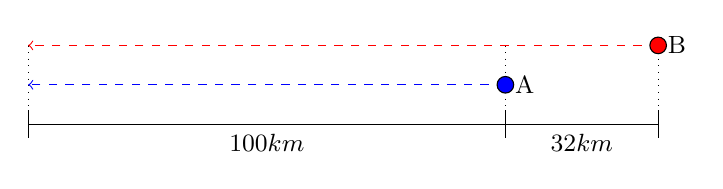
\begin{tikzpicture}[font=\small,x=10mm, y=10mm]
\draw (0,0) -- (8,0);
\foreach \x in {0,6.06,8}{
\draw (\x,5pt) -- (\x,-5pt);
\draw[dotted] (\x,1) -- (\x,0);
}

\draw[dashed, red, ->] (8,1) -- (0,1);
\draw[dashed, blue, ->] (6.06,.5) -- (0,.5);

\draw[fill=blue] (6.06,.5) circle (3pt) node [right] () {A};
\draw[fill=red] (8,1) circle (3pt) node [right] () {B};

\node[below] at (3.03,0) {$100\unit{km}$};
\node[below] at (7.03,0) {$32\unit{km}$};
\end{tikzpicture}
\end{center}
Traccia di soluzione:
\begin{itemize}
 \item se A e B partono insieme e arrivano insieme significa che hanno impiegato lo stesso tempo per fare il proprio viaggio;
 \item il tempo è dato dal rapporto tra lo spazio percorso e la velocità;
 \item la velocità di A è l’incognita del problema: la indichiamo con~$x$;
 \item l’equazione risolvente è~$\dfrac{110}{x}=\dfrac{132}{x+20}$.
\end{itemize}
Prosegui nella risoluzione.
\end{esercizio}

\begin{esercizio}
\label{ese:20.33}
Per percorrere~$480\unit{km}$ un treno impiega~$3$ ore di più di quanto impiegherebbe un aereo a percorrere~$\np[km]{1920}$.
L’aereo viaggia ad una velocità media che è~$8$ volte quella del treno. Qual è la velocità del treno?
\end{esercizio}

\subsubsection*{\thechapter.3 - Equazioni letterali}

\begin{esercizio}[\Ast]
\label{ese:20.34}
Risolvi e discuti le seguenti equazioni letterali nell'incognita~$x$.
\begin{multicols}{2}
\begin{enumeratea}
 \item $1+2x=a+1-2x$;
 \item $2x-\dfrac{7}{2}=ax-5$;
 \item $b^{2}x=2b+bx$;
 \item $ax+2=x+3$.
\end{enumeratea}
\end{multicols}
\end{esercizio}

\begin{esercizio}[\Ast]
\label{ese:20.35}
Risolvi e discuti le seguenti equazioni letterali nell'incognita~$x$.
\begin{multicols}{2}
\begin{enumeratea}
 \item $k(x+2)=k+2$;
 \item $(b+1)(x+1)=0$;
 \item $k^{2}x+2k=x+2$;
 \item $(a-1)(x+1)=x+1$.
\end{enumeratea}
\end{multicols}
\end{esercizio}

\begin{esercizio}
\label{ese:20.36}
Risolvi e discuti le seguenti equazioni letterali nell'incognita~$x$.
\begin{multicols}{2}
\begin{enumeratea}
 \item $ax+x-2a^{2}-2ax=0$;
 \item $3ax-2a=x\cdot (1-2a)+a\cdot (x-1)$;
 \item $x (3-5a)+2 (a-1)=(a-1) (a+1)$;
 \item $x+2a\cdot (x-2a)+1=0$.
\end{enumeratea}
\end{multicols}
\end{esercizio}
%\newpage
\begin{esercizio}[\Ast]
\label{ese:20.37}
Risolvi e discuti le seguenti equazioni letterali nell'incognita~$x$.
\begin{multicols}{2}
\begin{enumeratea}
 \item $(a-1)(x+1)=a-1$;
 \item $2k(x+1)-2=k(x+2)$;
 \item $a(a-1)x=2a(x-5)$;
 \item $3ax+a=2a^{2}-3a$.
\end{enumeratea}
\end{multicols}
\end{esercizio}

\begin{esercizio}[\Ast]
\label{ese:20.38}
Risolvi e discuti le seguenti equazioni letterali nell'incognita~$x$.
\begin{multicols}{2}
\begin{enumeratea}
 \item $3x-a=a(x-3)+6$;
 \item $2+2x=3ax+a-a^{2}x$;
 \item $x(a^{2}-4)=a+2$;
 \item $(x-m)(x+m)=(x+1)(x-1)$.
\end{enumeratea}
\end{multicols}
\end{esercizio}

\begin{esercizio}[\Ast]
\label{ese:20.39}
Risolvi e discuti le seguenti equazioni letterali nell'incognita~$x$.
\begin{multicols}{2}
\begin{enumeratea}
 \item $(a-2)^{2}x+(a-2)x+a-2=0$;
 \item $\left(9a^{2}-4\right)x=2(x+1)$;
 \item $(a-1)x=a^{2}-1$;
 \item $(a+2)x=a^{2}+a-1$.
\end{enumeratea}
\end{multicols}
\end{esercizio}

\begin{esercizio}[\Ast]
\label{ese:20.40}
Risolvi e discuti le seguenti equazioni letterali nell'incognita~$x$.
\begin{multicols}{2}
\begin{enumeratea}
 \item $a(x-1)^{2}=a(x^{2}-1)+2a$;
 \item $a^{3}x-a^{2}-4ax+4=0$;
 \item $bx\left(b^{2}+1\right)-(bx-1)\left(b^{2}-1\right)=2b^{2}$;
 \item $a(a-5)x+a(a+1)=-6(x-1)$:
 \item $(x+a)^{2}-(x-a)^{2}+(a-4)(a+4)=a^{2}$;
 \item $b(b+3)+x\left(6-b^{2}\right)=bx$.
\end{enumeratea}
\end{multicols}
\end{esercizio}

\begin{esercizio}[\Ast]
\label{ese:20.41}
Risolvi e discuti le seguenti equazioni nell'incognita~$x$ con due parametri.
\begin{multicols}{2}
\begin{enumeratea}
 \item $(m+1)(n-2)x=0$;
 \item $m(x-1)=n$;
 \item $(a+1)(b+1)x=0$;
 \item $(m+n)(x-1)=m-n$.
\end{enumeratea}
\end{multicols}
\end{esercizio}

\begin{esercizio}[\Ast]
\label{ese:20.42}
Risolvi e discuti le seguenti equazioni nell'incognita~$x$ con due parametri.
\begin{multicols}{2}
\begin{enumeratea}
 \item $x(2a-1)+2b(x-2)=-4a-x$;
 \item $ax-3+b=2(x+b)$;
 \item $(a+1)x=b+1$;
 \item $(a+b)(x-2)+3a-2b=2b(x-1)$.
\end{enumeratea}
\end{multicols}
\end{esercizio}

\begin{esercizio}[\Ast]
\label{ese:20.43}
Risolvi e discuti le seguenti equazioni nell'incognita~$x$ con due parametri.
\begin{enumeratea}
 \item $x(x+2)+3ax=b+x^{2}$;
 \item $(x-a)^{2}+b(2b+1)=(x-2a)^{2}+b-3a^{2}$.
\end{enumeratea}
\end{esercizio}

\begin{esercizio}[\Ast]
\label{ese:20.44}
Risolvi e discuti le seguenti equazioni che presentano il parametro al denominatore.
\begin{multicols}{2}
\begin{enumeratea}
 \item $\dfrac{x+2}{6a}+\dfrac{x-1}{2a^{2}}=\dfrac{1}{3a}$;
 \item $\dfrac{x-1}{b}+\dfrac{2x+3}{4b}=\dfrac{x}{4}$;
 \item $\dfrac{2x-1}{3a}+\dfrac{x}{3}=\dfrac{2}{a}$;
 \item $\dfrac{x}{a}+\dfrac{2x}{2-a}=\dfrac{a-x+2}{2a-a^{2}}$.
\end{enumeratea}
\end{multicols}
\end{esercizio}

\begin{esercizio}[\Ast]
\label{ese:20.45}
Risolvi e discuti le seguenti equazioni che presentano il parametro al denominatore.
\begin{multicols}{2}
\begin{enumeratea}
 \item $\dfrac{x}{a-1}+8=4a-\dfrac{x}{a-3}$;
 \item $\dfrac{x-1}{a-1}+\dfrac{x+a}{a}=\dfrac{a-1}{a}$;
 \item $\dfrac{a^{2}-9}{a+2}x=a-3$;
 \item $\dfrac{x+2}{a^{2}-2a}+\dfrac{x}{a^{2}+2a}+\dfrac{1}{a}=\dfrac{2}{a^{2}-4}$.
\end{enumeratea}
\end{multicols}
\end{esercizio}

\begin{esercizio}[\Ast]
\label{ese:20.46}
Risolvi e discuti le seguenti equazioni che presentano il parametro al denominatore.
\begin{enumeratea}
 \item $\dfrac{x+1}{a^{2}+2a+1}+\dfrac{2x+1}{a^{2}-a-2}-\dfrac{2x}{(a+1)(a-2)}+\dfrac{1}{a-2}=0$;
 \item $\dfrac{x+1}{a-5}+\dfrac{2x-1}{a-2}=\dfrac{2}{a^{2}-7a+10}$;
 \item $\dfrac{x+2}{b-2}+\dfrac{2}{b^{2}-4b+4}+\left(\dfrac{1}{b-2}+\dfrac{x}{b-1}\right)\cdot (b-1)=0$;
 \item $\dfrac{3+b^{3}x}{7b^{2}-b^{3}}+\dfrac{(2b^{2}+b)x+1}{b(b-7)}=\dfrac{3b^{2}x+1}{b^{2}}-2x$;
 \item $\dfrac{x-2}{t^{2}+3t}+\dfrac{x-1}{t+3}=\dfrac{x-2}{t^{2}}+\dfrac{1}{t+3}$;
 \item $\dfrac{x}{2a}+\dfrac{x+1}{1-2a}=\dfrac{1}{a}$.
\end{enumeratea}
\end{esercizio}

\begin{esercizio}[\Ast]
\label{ese:20.47}
Risolvi e discuti le seguenti equazioni parametriche frazionarie.
\begin{multicols}{2}
\begin{enumeratea}
 \item $\dfrac{t-1}{x-2}=2t$;
 \item $\dfrac{x+m}{x+1}=1$;
 \item $\dfrac{3}{x+1}=2a-1$;
 \item $\dfrac{2a-x}{x-3}-\dfrac{ax+2}{9-3x}=0$.
\end{enumeratea}
\end{multicols}
\end{esercizio}

\begin{esercizio}[\Ast]
\label{ese:20.48}
Risolvi e discuti le seguenti equazioni parametriche frazionarie.
\begin{multicols}{2}
\begin{enumeratea}
 \item $\dfrac{k-1}{x}=\dfrac{2}{k+1}$;
 \item $\dfrac{k}{x+1}=\dfrac{2k}{x-1}$;
 \item $\dfrac{a-1}{x+3}-\dfrac{a}{2-x}=\dfrac{ax+3a}{x^{2}+x-6}$;
 \item $\dfrac{a}{x}=\dfrac{1}{a}$.
\end{enumeratea}
\end{multicols}
\end{esercizio}

\begin{esercizio}[\Ast]
\label{ese:20.49}
Risolvi e discuti le seguenti equazioni parametriche frazionarie.
\begin{enumeratea}
 \item $\dfrac{x-a}{x^{2}-1}-\dfrac{x+3a}{2x-x^{2}-1}=\dfrac{x+5}{x+1}-2\dfrac{x}{(x-1)^{2}}-1$;
 \item $\dfrac{3}{1+3x}+\dfrac{a}{3x-1}=\dfrac{a-5x}{1-9x^{2}}$;
 \item $\dfrac{2a}{x^{2}-x-2}+\dfrac{1}{3x^{2}+2x-1}=\dfrac{6a^{2}-13a-4}{3x^{3}-4x^{2}-5x+2}$;
 \item $\dfrac{a+1}{x+1}-\dfrac{2a}{x-2}=\dfrac{3-5a}{x^{2}-x-2}$.
\end{enumeratea}
\end{esercizio}

\begin{esercizio}[\Ast]
\label{ese:20.50}
Risolvi e discuti le seguenti equazioni parametriche frazionarie.
\begin{multicols}{2}
\begin{enumeratea}
 \item $\dfrac{a}{x+a}=1+a$;
 \item $\dfrac{x}{x-a}+\dfrac{1}{x+a}=1$;
 \item $\dfrac{x+a}{x-a}=\dfrac{x-a}{x+a}$;
 \item $\dfrac{2}{1-ax}+\dfrac{1}{2+ax}=0$.
\end{enumeratea}
\end{multicols}
\end{esercizio}

\begin{esercizio}[\Ast]
\label{ese:20.51}
Risolvi e discuti le seguenti equazioni parametriche frazionarie.
\begin{multicols}{2}
\begin{enumeratea}
 \item $\dfrac{2}{x-2}+\dfrac{a+1}{a-1}=0$;
 \item $\dfrac{1}{x+t}-\dfrac{1}{t+1}=\dfrac{tx}{tx+x+t^{2}+t}$;
 \item $\dfrac{tx}{x-2}+\dfrac{t^{2}}{t+1}-\dfrac{t}{x-2}=0$;
 \item $\dfrac{2x+1}{2x-1}=\dfrac{2a-1}{a+1}$.
\end{enumeratea}
\end{multicols}
\end{esercizio}

\begin{esercizio}
\label{ese:20.52}
Risolvi e discuti le seguenti equazioni parametriche frazionarie.
\begin{multicols}{2}
\begin{enumeratea}
 \item $\dfrac{a}{x+1}=\dfrac{3}{x-2}$;
 \item $\dfrac{x}{x+1}+\dfrac{x}{x-1}=\dfrac{bx}{1-x^{2}}+\dfrac{a+2x^{2}}{x^{2}-1}$;
 \item $\dfrac{2x+1}{x}+\dfrac{2x^{2}-3b^{2}}{bx-x^{2}}=\dfrac{1}{x-b}$;
 \item $\dfrac{x-1}{x+a}=2+\dfrac{1-x}{x-a}$.
\end{enumeratea}
\end{multicols}
\end{esercizio}

\subsubsection*{20.4 - Equazioni letterali e formule inverse}

\begin{esercizio}
\label{ese:20.53}
L'interesse~$I$ maturato da un capitale~$C$, al tasso di interesse annuo~$i$, per un numero di anni~$t$ è
\begin{equation*}
  I=C\cdot i\cdot t.
\end{equation*}

Ricava le formule per calcolare:~$C=\ldots\ldots\ldots\ldots$, $\quad i=\ldots\ldots\ldots\ldots$, $\quad t =\ldots\ldots\ldots\ldots$.

Se il capitale è \officialeuro~$\np{12000}$, il tasso di interesse annuo~$\np{3,5}\%$, il periodo di tempo è di~$6$ anni, calcola~$I$.
\end{esercizio}

\begin{esercizio}
\label{ese:20.54}
Conversione da gradi Celsius $C$ a gradi Fahrenheit $F$:
\begin{equation*}
  C=\frac{5(F-32)}{9}.
\end{equation*}

Ricava la formula per calcolare $F=\ldots\ldots\ldots\ldots$.

Calcola il valore di~$C$ quando~$F$ vale~$106$ e il valore di~$F$ quando~$C$ vale~$12$.
\end{esercizio}

\begin{esercizio}
\label{ese:20.55}
Il valore attuale~$V_a$ di una rendita che vale~$V_n$ dopo~$n$ anni al tasso di interesse~$i$, anticipata di~$t$ anni è
\begin{equation*}
  V_{a}=V_{n}\cdot (1-i\cdot t).
\end{equation*}

Ricava le formule per calcolare:~$V_n=\ldots\ldots\ldots\ldots$, $\quad i=\ldots\ldots\ldots\ldots$, $\quad t =\ldots\ldots\ldots\ldots$.

Se il valore attuale è \officialeuro~$\np{120000}$, il tasso di interesse il~$2\%$, calcola il valore della rendita dopo~$20$ anni.
\end{esercizio}

\begin{esercizio}
\label{ese:20.56}
Lo sconto semplice~$S$, per un montante~$M$, al tasso di interesse~$i$, per un tempo di~$t$ anni è:
\begin{equation*}
  S=\frac{M\cdot i\cdot t}{1+i\cdot t}.
\end{equation*}

Ricava le formule per calcolare:~$M=\ldots\ldots\ldots\ldots$, $\quad i=\ldots\ldots\ldots\ldots$.

Se lo sconto semplice è \officialeuro~$\np{12000}$, il tempo è~$12$ anni, il tasso di interesse il~$\np{4,5}\%$, calcola il montante.
\end{esercizio}

\begin{esercizio}
\label{ese:20.57}
La superficie~$S$ di un trapezio con base maggiore~$B$, base minore~$b$ e altezza~$h$ è
\begin{equation*}
  S=\frac{1}{2}\cdot (B+b)\cdot h.
\end{equation*}

Ricava le formule per calcolare:~$B=\ldots\ldots\ldots\ldots$, $\quad b=\ldots\ldots\ldots\ldots$, $\quad h =\ldots\ldots\ldots\ldots$.

Se la base maggiore è~$12\unit{cm}$, la base minore~$8\unit{cm}$, la superficie~$12\unit{cm^2}$, calcola l'altezza del trapezio.
\end{esercizio}

\begin{esercizio}
\label{ese:20.58}
La superficie laterale~$S_l$ di un tronco di piramide con perimetro della base maggiore~$2p_B$, perimetro della base minore~$2p_b$ e apotema~$a$
($2p_B$ e~$2p_b$ sono da considerare come un'unica incognita):
\begin{equation*}
  S_{l}=\frac{(2p_B+2p_b)\cdot a}{2}.
\end{equation*}

Ricava le formule per calcolare:~$2p_B=\ldots\ldots\ldots\ldots$, $\quad~2p_b=\ldots\ldots\ldots\ldots$, $\quad a =\ldots\ldots\ldots$.

Se la superficie laterale vale~$144\unit{cm^2}$, il perimetro della base minore~$12\unit{cm}$ e il perimetro della base maggiore~$14\unit{cm}$, calcola l'apotema.
\end{esercizio}

\begin{esercizio}
\label{ese:20.59}
Il volume~$V$ del segmento sferico con una base di raggio~$r$ e altezza~$h$ è
\begin{equation*}
  V=\pi \cdot h^{2}\cdot \left(r-\frac{h}{3}\right).
\end{equation*}

Ricava la formula per calcolare~$r=\ldots\ldots\ldots\ldots$.

Se il volume misura~$200\unit{cm^3}$ e l'altezza~$10\unit{cm}$, calcola la misura del raggio.
\end{esercizio}

\begin{esercizio}
\label{ese:20.60}
La superficie totale~$S$ del cono con raggio di base~$r$ e apotema~$a$ è
\begin{equation*}
  S=\pi \cdot r\cdot (r+a).
\end{equation*}

Ricava la formula per calcolare~$a=\ldots\ldots\ldots\ldots$.

Se la superficie totale è~$98\unit{cm^2}$ e il raggio di base~$6\unit{cm}$, calcola la misura dell'apotema.
\end{esercizio}

\begin{esercizio}
\label{ese:20.61}
La velocità~$v$ di un corpo che si muove di moto rettilineo uniformemente accelerato con velocità iniziale~$v_0$ e accelerazione costante~$a$, dopo un tempo~$t$ è
\begin{equation*}
  v=v_{0}+a\cdot t.
\end{equation*}

Ricava le formule per calcolare:~$v_0=\ldots\ldots\ldots\ldots$, $\quad a=\ldots\ldots\ldots\ldots$, $\quad t =\ldots\ldots\ldots\ldots$.

Se un corpo è passato in~$10$ secondi dalla velocità (iniziale) di~$10\unit{m/s}$ alla velocità di~$24\unit{m/s}$, qual è stata la sua accelerazione?
\end{esercizio}

\begin{esercizio}
\label{ese:20.62}
Lo spazio~$s$ percorso da un corpo che si muove di moto rettilineo uniformemente accelerato con posizione iniziale~$s_0$,
 velocità iniziale~$v_0$ e accelerazione~$a$, dopo un intervallo di tempo~$t$ è
\begin{equation*}
  s=s_{0}+v_{0}\cdot t+\dfrac{1}{2}\cdot a\cdot t^{2}.
\end{equation*}

Ricava le formule per calcolare:~$v_0=\ldots\ldots\ldots\ldots$, $\quad a=\ldots\ldots\ldots\ldots$.

Se un corpo ha percorso~$100\unit{m}$, partendo dalla posizione iniziale~$0$, accelerazione~$3\unit{m/s^2}$, in~$10$ secondi, qual era la sua velocità iniziale?
\end{esercizio}

\begin{esercizio}
\label{ese:20.63}
La formula di Bernoulli relativa al moto di un fluido è
\begin{equation*}
  p+\rho \cdot g\cdot h+\dfrac{1}{2}\rho \cdot v^{2}=k.
\end{equation*}

Ricava le formule per calcolare:~$h=\ldots\ldots\ldots\ldots$, $\quad \rho=\ldots\ldots\ldots\ldots$.
\end{esercizio}

\begin{esercizio}
\label{ese:20.64}
La seconda legge di Gay-Lussac per i gas è
\begin{equation*}
  V=V_{0}\cdot (1+\alpha \cdot t).
\end{equation*}

Ricava le formule per calcolare:~$V_0=\ldots\ldots\ldots\ldots$, $\quad t=\ldots\ldots\ldots\ldots$.
\end{esercizio}

\begin{esercizio}
\label{ese:20.65}
L'equazione di stato dei gas perfetti è
\begin{equation*}
  pV=nRT.
\end{equation*}

Ricava le formule per calcolare:~$V=\ldots\ldots\ldots\ldots$, $\quad T=\ldots\ldots\ldots\ldots$.
\end{esercizio}

\begin{esercizio}
\label{ese:20.66}
Il rendimento del ciclo di Carnot è
\begin{equation*}
  \eta =1-\dfrac{T_{1}}{T_{2}}.
\end{equation*}

Ricava le formule per calcolare:~$T_1=\ldots\ldots\ldots\ldots$, $\quad T_2=\ldots\ldots\ldots\ldots$.
\end{esercizio}

\begin{esercizio}
\label{ese:20.67}
La legge di Stevino è
\begin{equation*}
  P_{B}=P_{A}+\rho \cdot g\cdot (z_{A}-z_{B}).
\end{equation*}

Ricava le formule per calcolare:~$\rho=\ldots\ldots\ldots\ldots$, $\quad z_A=\ldots\ldots\ldots\ldots$, $\quad z_B =\ldots\ldots\ldots\ldots$.
\end{esercizio}

\begin{esercizio}
\label{ese:20.68}
Risolvi le seguenti equazioni rispetto alla lettera richiesta.
\begin{multicols}{2}
\TabPositions{2.5cm}
\begin{enumeratea}
 \item $y=\dfrac{2-a}{x}$\tab$x=\ldots$, $a=\ldots$;
 \item $y=2-\dfrac{a}{x}$\tab$x=\ldots$, $a=\ldots$;
 \item $y=\dfrac{2}{x}-a$\tab$x=\ldots$, $a=\ldots$;
 \item $y=-{\dfrac{2-a}{x}}$\tab$x=\ldots$, $a=\ldots$.
\end{enumeratea}
\end{multicols}
\end{esercizio}

\begin{esercizio}
\label{ese:20.69}
Risolvi le seguenti equazioni rispetto alla lettera richiesta.
\begin{multicols}{2}
\TabPositions{3.5cm}
\begin{enumeratea}
 \item $\dfrac{2x+1}{2x-1}=\dfrac{2k-1}{k+1}$\tab$k=\ldots$;
 \item $(m-1)x=m-3$\tab$m=\ldots$;
 \item $\dfrac{2}{x+2}+\dfrac{a-1}{a+1}=0$\tab$a=\ldots$;
 \item $(a+1)(b-1)x=0$\tab$b=\ldots$.
\end{enumeratea}
\end{multicols}
\end{esercizio}

\begin{esercizio}[\Ast]
\label{ese:20.70}
Risolvi le seguenti equazioni rispetto alla lettera richiesta.
\TabPositions{5cm}
\begin{enumeratea}
 \item $\dfrac{x}{a+b}+\dfrac{x-b}{a-b}=\dfrac{b}{a^{2}-b^{2}}$\tab$a=\ldots$, $x=\ldots$;
 \item $\dfrac{2x}{a+b}+\dfrac{bx}{a^{2}-b^{2}}-\dfrac{1}{a-b}=0$\tab$a=\ldots$, $b=\ldots$.
\end{enumeratea}
\end{esercizio}

\subsection{Risposte}
\begin{multicols}{2}
 \paragraph{\thechapter.1.}
a)~$\{0\text{,~}-2\}$;\quad b)~$\{-2\text{,~}+9\}$;\quad c)~$\{2\text{,~}-1\}$;\quad d)~$\{-2\}$.
\paragraph{\thechapter.2.}
a)~$\{5\text{,~}-2\}$;\quad b)~$\{2\text{,~}-6\}$;\quad c)~$\{3\text{,~}-1\}$;\quad d)~$\{2\text{,~}-7\}$.
\paragraph{\thechapter.3.}
a)~$\{2\text{,~}-5\}$;\quad b)~$\{7\text{,~}-6\}$;\quad c)~$\{4\text{,~}-6\}$;\quad d)~$\{6\text{,~}-8\}$.
\paragraph{\thechapter.4.}
a)~$\{0\text{,~}+4\text{,~}-4\}$;\quad b)~$\{1\text{,~}+2\text{,~}-4\}$;\quad c)~$\{2\text{,~}-1\}$;\quad d)~$\{0\text{,~}+2\text{,~}+5\}$.
\paragraph{\thechapter.5.}
a)~$\{1\text{,~}+5\text{,~}-3\}$;\quad b)~$\{2\text{,~}-12\}$;\quad c)~$\{0\text{,~}-3\text{,~}+4\}$;\quad d)~$\{1\text{,~}-1\text{,~}+2\text{,~}-2\}$.
\paragraph{\thechapter.6.}
a)~$\{-5\}$;\quad b)~$\{0\text{,~}+1\text{,~}-1\}$;\quad c)~$\{0\text{,~}+1\text{,~}-8\}$;\quad d)~$\{-1\text{,~}+3\text{,~}-3\}$.
\paragraph{\thechapter.7.}
a)~$\{1\text{,~}+9\text{,~}-5\}$;\quad b)~$\{-1\text{,~}+4\text{,~}-4\}$;\quad c)~$\{1\text{,~}-1\text{,~}+6\}$;\quad d)~$\{2\text{,~}-2\}$.
\paragraph{\thechapter.8.}
a)~$\{-1\text{,~}-2\text{,~}-8\}$;\quad b)~$\{4\text{,~}-4\text{,~}-3\}$,\quad c)~$\{1\text{,~}-1\text{,~}-8\}$;\quad d)~$\{7\}$.
\paragraph{\thechapter.9.}
a)~$\{-6\}$;\quad b)~$\{1\text{,~}+2\text{,~}+3\text{,~}+4\}$;\quad c)~$\{-1\text{,~}+2\text{,~}-7\}$;\quad d)~$\{1\text{,~}-1\text{,~}-4\text{,~}+6\}$.

\paragraph{\thechapter.10.}
a)~$\{1\text{,~}-2\text{,~}+5\text{,~}-4\}$;\quad b)~$\{0\text{,~}+1\text{,~}+2\text{,~}+4\}$;\quad c)~$\left\{\frac{5}{2}\text{,~}-\frac{5}{2}\text{,~}\frac{2}{3}\right\}$;\quad d)~$\{4\text{,~}+2\text{,~}-2\}$.

\paragraph{\thechapter.11.}
a)~$\{0\text{,~}+1\text{,~}-1\text{,~}+3\text{,~}-3\}$;\quad b)~$\{1\text{,~}-1\text{,~}-2\text{,~}+3\text{,~}-4\}$;\quad c)~$\left\{1\text{,~}-\frac{1}{2}\right\}$;\quad d)~$\left\{-2\text{,~}\frac{1}{3}\right\}$.

\paragraph{\thechapter.12.}
a)~$\left\{\frac{1}{2}\text{,~}-\frac{2}{3}\right\}$;\quad b)~$\left\{1\text{,~}-1\text{,~}\frac{1}{2}\right\}$;\quad c)~$\left\{-1\text{,~}2\text{,~}-\frac{2}{3}\right\}$;\quad d)~$\left\{-1\text{,~}-\frac{1}{2}\text{,~}\frac{3}{4}\right\}$.

\paragraph{\thechapter.13.}
a)~$\left\{1\text{,~}\frac{1}{3}\text{,~}-\frac{3}{2}\right\}$;\quad b)~$\left\{3\text{,~}-1\text{,~}\frac{1}{2}\text{,~}-\frac{1}{2}\right\}$;\quad c)~$\left\{2\text{,~}-2\text{,~}\frac{3}{4}\text{,~}\frac{1}{2}\right\}$;\quad d)~$\left\{5\text{,~}\frac{1}{2}\text{,~}\frac{1}{6}\right\}$.

\paragraph{\thechapter.14.}
$\{-1\text{,~}+2\text{,~}+3\text{,~}-3\}$.

\paragraph{\thechapter.15.}
a)~$\{-3\}$;\quad b)~$\left\{\frac{3}{2}\right\}$;\quad c)~$\{0\}$;\quad d)~$\emptyset$.

\paragraph{\thechapter.16.}
a)~$\{0\}$;\quad b)~$\{-1\}$;\quad c)~$\left\{\frac{11}{6}\right\}$;\quad d)~$\emptyset$.

\paragraph{\thechapter.17.}
a)~$\emptyset$;\quad b)~$\{-1\}$;\quad c)~$\emptyset$;\quad d)~$\{2\text{,~}-1\}$.

\paragraph{\thechapter.18.}
a)~$\left\{\frac{3}{2}\right\}$;\quad b)~$\{0\text{,~}-3\}$;\quad c)~$\{1\}$;\quad d)~$\{-2\}$.

\paragraph{\thechapter.19.}
a)~$\emptyset$;\quad b)~$\left\{\frac{9}{2}\right\}$;\quad c)~$\{-1\}$;\quad d)~$\left\{-{\frac{1}{3}}\right\}$.

\paragraph{\thechapter.20.}
a)~$\{-1\}$;\quad b)~$\left\{\frac{1}{3}\right\}$;\quad c)~$\emptyset$;\quad d)~$\{1\text{,~}-2\}$.

\paragraph{\thechapter.21.}
a)~$\left\{\frac{2}{25}\right\}$;\quad b)~$\emptyset$;\quad c)~$\emptyset$;\quad d)~$\left\{-{\frac{1}{3}}\right\}$.

\paragraph{\thechapter.22.}
a)~$\left\{\frac{3}{4}\right\}$;\quad b)~$\left\{\frac{7}{3}\right\}$;\quad c)~$\emptyset$;\quad d)~$\emptyset$.

\paragraph{\thechapter.23.}
a)~$\insR-\{2\}$;\quad b)~$\left\{-{\frac{3}{2}}\text{,~}\frac{5}{3}\right\}$;\quad c)~$\{-5\}$;\quad d)~$\{4\text{,~}-3\text{,~}3\}$.

\paragraph{\thechapter.24.}
a)~$\insR-\left\{-{\frac{2}{3}}\text{,~}2\right\}$;\quad b)~$\{1\}$;\quad c)~$\left\{-{\frac{2}{3}}\right\}$;\quad d)~$\{1\}$.

\paragraph{\thechapter.25.}
a)~$\left\{\frac{1}{2}\right\}$;\quad b)~$\{2\text{,~}3\}$;\quad c)~$\left\{-\frac{2}{3}\right\}$;\quad d)~$\{2\}$.

\paragraph{\thechapter.26.}
a)~$\{-5,+1\}$;\quad b)~$\left\{2\text{,~}-\frac{1}{4}\text{,~}-2\right\}$;\quad c)~$\emptyset$;\quad d)~$\left\{-{\frac{3}{16}}\right\}$.

\paragraph{\thechapter.27.}
a)~$\insR-\{-3\}$;\quad b)~$\left\{\frac{3}{2}\right\}$;\quad c)~$\left\{\frac{35}{3}\right\}$;\quad d)~$\left\{-{\frac{3}{4}}\right\}$.

\paragraph{\thechapter.28.}
a)~$\left\{\frac{5}{3}\right\}$;\quad b)~$\left\{-\frac{4}{3}\right\}$;\quad c)~$\{4\}$;\quad d)~$\left\{-{\frac{26}{25}}\right\}$;\quad e)~$\left\{\frac{12}{5}\right\}$;\quad f)~$\{-30\}$.

\paragraph{\thechapter.30.} $x=21$

\paragraph{\thechapter.31.} $x=28$
\end{multicols}
\paragraph{\thechapter.34.}
a)~$\forall a\in \insR \rightarrow \left\{\frac{a}{4}\right\}$;
\quad b)~$a=2 \rightarrow \emptyset$, $a\neq~2 \rightarrow \left\{\frac{3}{2(a-2)}\right\}$;
\quad \protect\\
c)~$b=0 \rightarrow \insR$, $b=1\rightarrow\emptyset$, $b\neq~0\wedge b\neq~1\rightarrow \left\{\frac{2}{b-1}\right\}$;
\quad d)~$a=1\rightarrow \emptyset$, $a\neq~1\rightarrow \left\{\frac{1}{a-1}\right\}$.

\paragraph{\thechapter.35.}
a)~$k=0 \rightarrow \emptyset$, $k\neq~0 \rightarrow \left\{\frac{2-k}{k}\right\}$;
\quad b)~$b=-1 \rightarrow \insR$, $b\neq -1 \rightarrow \left\{-1\right\}$;
\quad \protect\\
c)~$k=1 \rightarrow \insR$, $k=-1 \rightarrow \emptyset$, $k\neq~1\wedge k\neq -1 \rightarrow \left\{-{\frac{2}{k+1}}\right\}$;
\quad d)~$a=2 \rightarrow \insR$, $a\neq~2 \rightarrow \left\{-1\right\}$.

\paragraph{\thechapter.37.}
a)~$a=1 \rightarrow \insR$, $a\neq~1 \rightarrow \{0\}$;
\quad b)~$k=0 \rightarrow \emptyset$, $k\neq~0 \rightarrow \left\{\frac{2}{k}\right\}$;
\quad \protect\\
c)~$a=0 \rightarrow \insR$, $a=3\rightarrow \emptyset$, $a\neq~0 \wedge a\neq~3 \rightarrow \left\{\frac{10}{3-a}\right\}$;
\quad d)~$a=0 \rightarrow \insR$, $a\neq~0 \rightarrow \left\{\frac{2}{3} (a-2)\right\}$.

\paragraph{\thechapter.38.}
a)~$a=3 \rightarrow \insR$, $a\neq~3 \rightarrow \{2\}$;
\quad b)~$a=2 \rightarrow \insR$, $a=1 \rightarrow \emptyset$, $a\neq~2\wedge a\neq~1 \rightarrow \left\{\frac{1}{a-1}\right\}$;
\quad c)~$a=2 \rightarrow \emptyset$, $a=-2 \rightarrow \insR$, $a\neq -2\wedge a\neq~2 \rightarrow \left\{\frac{1}{a-2}\right\}$;
\quad\protect\\
d)~$m=1\vee m=-1 \rightarrow \insR$, $m\neq~1\wedge m\neq -1 \rightarrow \emptyset$.

\paragraph{\thechapter.39.}
a)~$a=2 \rightarrow \insR$, $a=1 \rightarrow \emptyset$, $a\neq~1\wedge a\neq~2 \rightarrow \left\{\frac{1}{1-a}\right\}$;
\quad\protect\\
b)~$3a^{2}-2=0 \rightarrow \emptyset$, $3a^{2}-2\neq~0 \rightarrow \left\{\frac{2}{3(3a^{2}-2)}\right\}$;
\quad c)~$a=1 \rightarrow \insR$, $a\neq~1 \rightarrow \{a+1\}$;
\quad d)~$a=-2 \rightarrow \emptyset$, $a\neq -2 \rightarrow \left\{\frac{a^{2}+a-1}{a+2}\right\}$.

\paragraph{\thechapter.40.}
a)~$a=0 \rightarrow \insR$, $a\neq~0 \rightarrow \{0\}$;
\quad \protect\\
b)~$a=-2\vee a=2 \rightarrow \insR$, $a=0 \rightarrow \emptyset$, $a\neq -2\wedge a\neq~0\wedge a\neq~2 \rightarrow \left\{\frac{1}{a}\right\}$;
\quad\protect\\
c)~$b=0 \rightarrow \emptyset$, $b\neq~0 \rightarrow \left\{\frac{1+b^{2}}{2b}\right\}$;
\quad d)~$a=2 \rightarrow \insR$, $a=3 \rightarrow \emptyset$, $a\neq~2\wedge a\neq~3 \rightarrow \left\{\frac{a+3}{3-a}\right\}$;
\quad e)~$a=0 \rightarrow \emptyset$, $a\neq~0 \rightarrow \left\{\frac{4}{a}\right\}$;
\quad f)~$b=-3 \rightarrow \insR$, $b=2 \rightarrow \emptyset$, $b\neq -3\wedge b\neq~2 \rightarrow \left\{\frac{b}{b-2}\right\}$.

\paragraph{\thechapter.41.}
a)~$m=-1\vee n=2 \rightarrow \insR$, $m\neq -1\wedge n\neq~2 \rightarrow \{0\}$;
\protect\\
b)~$m=0\wedge n\neq~0 \rightarrow \emptyset$, $m=0\wedge n=0 \rightarrow \insR$, $m\neq~0 \rightarrow \left\{\frac{m+n}{m}\right\}$;
\protect\\
c)~$a=-1\vee b=-1 \rightarrow \insR$, $a\neq -1\wedge b\neq -1 \rightarrow \{0\}$;
\protect\\ d)~$m=n=0 \rightarrow \insR$, $m=-n\neq~0 \rightarrow \emptyset$, $m\neq -n \rightarrow \left\{\frac{2m}{m+n}\right\}$.

\paragraph{\thechapter.42.}
a)~$a=b=0 \rightarrow \insR$, $a=-b\neq~0 \rightarrow \emptyset$, $a\neq -b \rightarrow \left\{\frac{2(b-a)}{a+b}\right\}$;
\protect\\ b)~$a=2\wedge b=-3 \rightarrow \insR$, $a=2\wedge b\neq -3 \rightarrow \emptyset$, $a\neq~2 \rightarrow \left\{\frac{b+3}{a-2}\right\}$;
\protect\\ c)~$a=-1\wedge b=-1 \rightarrow \insR$, $a=-1\wedge b\neq -1 \rightarrow \emptyset$, $a\neq -1 \rightarrow \left\{\frac{b+1}{a+1}\right\}$;
\protect\\ d)~$a=b=0 \rightarrow \insR$, $a=b\neq~0 \rightarrow \emptyset$, $a\neq b \rightarrow \left\{\frac{2b-a}{a-b}\right\}$.

\paragraph{\thechapter.43.}
a)~$a=-{\frac{2}{3}}\wedge b=0 \rightarrow \insR$, $a=-{\frac{2}{3}}\wedge b\neq~0 \rightarrow \emptyset$, $a\neq -{\frac{2}{3}} \rightarrow \left\{\frac{b}{2+3a}\right\}$;
\protect\\ b)~$a=0\wedge b=0 \rightarrow \insR$, $a=0\wedge b\neq~0 \rightarrow \emptyset$, $a\neq~0 \rightarrow \left\{-{\frac{b^{2}}{a}}\right\}$.

\paragraph{\thechapter.44.}
a)~$a=0 \rightarrow$ assurdo, $a=-3 \rightarrow \emptyset$, $a\neq~0\wedge a\neq -3 \rightarrow \left\{\frac{3}{a+3}\right\}$;
\protect\\ b)~$b=0 \rightarrow$ assurdo, $b=6 \rightarrow \emptyset$, $b\neq~0\wedge b\neq~6 \rightarrow \left\{\frac{1}{6-b}\right\}$;
\protect\\ c)~$a=0 \rightarrow$ assurdo, $a=-2 \rightarrow \emptyset$, $a\neq~0\wedge a\neq -2 \rightarrow \left\{\frac{7}{2+a}\right\}$;
\protect\\ d)~$a=0\vee a=2 \rightarrow$ assurdo, $a=-3 \rightarrow \emptyset$, $a\neq~0\wedge a\neq~2\wedge a\neq -3 \rightarrow \left\{\frac{a+2}{a+3}\right\}$.

\paragraph{\thechapter.45.}
a)~$a=1\vee a=3 \rightarrow$ assurdo, $a\neq~1\wedge a\neq~3 \rightarrow \{2(a-1)(a-3)\}$;
\protect\\ b)~$a=0\vee a=1 \rightarrow$ assurdo, $a=\frac{1}{2} \rightarrow \emptyset$, $a\neq~0\wedge a\neq \frac{1}{2}\wedge a\neq~1 \rightarrow \left\{\frac{1}{2a-1}\right\}$;
\protect\\ c)~$a=-2 \rightarrow$ assurdo, $a=-3 \rightarrow \emptyset$, $a=3 \rightarrow \insR$, $a\neq -3\wedge a\neq -2\wedge a\neq~3 \rightarrow \left\{\frac{a+2}{a+3}\right\}$;
\protect\\ d)~$a=0\vee a=-2\vee a=2 \rightarrow$ assurdo, $a\neq~0\wedge a\neq -2\wedge a\neq~2 \rightarrow \left\{-{\frac{a}{2}}\right\}$.

\paragraph{\thechapter.46.}
a)~$a=2\vee a=-1 \rightarrow$ assurdo, $a\neq~2\wedge a\neq -1 \rightarrow \left\{\frac{a(a+4)}{2-a}\right\}$;
\protect\\ b)~$a=5\vee a=2 \rightarrow$ assurdo, $a=4 \rightarrow \emptyset$, $a\neq~5\wedge a\neq~2\wedge a\neq~4 \rightarrow \left\{\frac{1}{3(4-a)}\right\}$;
\protect\\ c)~$b=2\vee b=1 \rightarrow$ assurdo, $b\neq~2\wedge b\neq~1 \rightarrow \left\{\frac{b}{2-b}\right\}$;
\protect\\ d)~$b=0\vee b=7\rightarrow$ assurdo, $b\neq~0\wedge b\neq~7 \rightarrow \left\{-{\frac{1}{2b^{2}}}\right\}$;
\protect\\ e)~$t=0\vee t=-3 \rightarrow$ assurdo, $t^{2}=3 \rightarrow \insR$, $t\neq~0\wedge t\neq -3\wedge t^{2}\neq~3 \rightarrow \{2\}$;
\protect\\ f)~$a=0\vee a=\frac{1}{2} \rightarrow$ assurdo, $a\neq~0\wedge a\neq \frac{1}{2} \rightarrow \{2-6a\}$.

\paragraph{\thechapter.47.}
a)~$t=0\vee t=1 \rightarrow \emptyset$, $t\neq~0\wedge t\neq~1 \rightarrow \left\{\frac{5t-1}{2t}\right\}$;
\quad b)~$m=1 \rightarrow \insR-\{-1\}$, $m\neq~1 \rightarrow \emptyset$;
\quad c)~$a=\frac{1}{2} \rightarrow \emptyset$, $a\neq \frac{1}{2} \rightarrow \left\{-{\frac{2(a-2)}{2a-1}}\right\}$;
\protect\\ d)~$a=3\vee a=\frac{7}{9} \rightarrow \emptyset$, $a\neq~3\wedge a\neq \frac{7}{9} \rightarrow \left\{\frac{2(3a+1)}{3-a}\right\}$.

\paragraph{\thechapter.48.}
a)~$k=-1 \rightarrow$ assurdo, $k=1 \rightarrow \emptyset$, $k\neq~1\wedge k\neq -1 \rightarrow \left\{-{\frac{\left(k^2-1\right)}{2}}\right\}$;
\protect\\ b)~$k=0 \rightarrow \insR-\{1\text{,~}-1\}$ $k\neq~0 \rightarrow \{-3\}$; c)~$a=1 \rightarrow \insR-\{-3\text{,~}2\}$, $a\neq~1 \rightarrow \emptyset$;
\protect\\ d)~$a=0 \rightarrow$ assurdo, $a\neq~0 \rightarrow \left\{a^{2}\right\}$.

\paragraph{\thechapter.49.}
a)~$a=-5\vee a=-1\vee a=7 \rightarrow \emptyset$, $a\neq -5\wedge a\neq -1\wedge a\neq~7 \rightarrow \left\{\frac{-2(a-1)}{a+5}\right\}$;
\quad b)~$a=-{\frac{4}{3}}\vee a=\frac{5}{9}\vee a=\frac{13}{3} \rightarrow \emptyset$, $a\neq -{\frac{4}{3}}\wedge a\neq \frac{5}{9}\wedge a\neq \frac{13}{3} \rightarrow \left\{\frac{3-2a}{4+3a}\right\}$;
\protect\\ c)~$a=-{\frac{1}{6}} \rightarrow \insR-\left\{-1\text{,~}2\text{,~}\frac{1}{3}\right\}$, $a=\frac{7}{3}\vee a=4\vee a=1 \rightarrow \emptyset$, $a\neq -{\frac{1}{6}}\wedge a\neq \frac{7}{3}\wedge a\neq~4\wedge a\neq~1 \rightarrow \{a-2\}$;
\quad d)~$a=1\vee a=-3\vee a=3 \rightarrow \emptyset$, $a\neq -3\wedge a\neq~1\wedge a\neq~3 \rightarrow \left\{\frac{5-a}{1-a}\right\}$.

\paragraph{\thechapter.50.}
a)~$a=-1\vee a=0 \rightarrow \emptyset$, $a\neq -1\wedge a\neq~0 \rightarrow \left\{-{\frac{\ a^{2}}{1+a}}\right\}$;
\protect\\ b)~$a=-1\vee a=0 \rightarrow \emptyset$, $a\neq -1\wedge a\neq~0 \rightarrow \left\{-{\frac{a(a-1)}{a+1}}\right\}$;
\quad c)~$a=0 \rightarrow \insR-\{0\}$, $a\neq~0 \rightarrow \{0\}$;
\quad d)~$a=0 \rightarrow \emptyset$, $a\neq~0 \rightarrow \left\{-{\frac{5}{a}}\right\}$.

\paragraph{\thechapter.51.}
a)~$a=1 \rightarrow$ assurdo, $a=-1 \rightarrow \emptyset$, $a\neq~1\wedge a\neq -1 \rightarrow \left\{\frac{4}{a+1}\right\}$;
\protect\\ b)~$t=-1 \rightarrow$ assurdo, $t\neq -1 \rightarrow \left\{\frac{1}{t+1}\right\}$;
\protect\\ c)~$t=-1 \rightarrow$ assurdo, $t=0 \rightarrow \insR-\{2\}$, $t=-{\frac{1}{2}} \rightarrow \emptyset$, $t\neq -\frac{1}{2}\wedge t\neq -1\wedge t\neq~0 \rightarrow \left\{\frac{3t+1}{2t+1}\right\}$;
\quad d)~$a=-1 \rightarrow$ assurdo, $a=2 \rightarrow \emptyset$, $a\neq -1\wedge a\neq~2 \rightarrow \left\{\frac{3a}{2(a-2)}\right\}$.

\paragraph{\thechapter.70.}
a)~$a=\frac{b(b+1)}{2x-b}$, $x=\frac{b(a+b+1)}{2a}$;
\quad b)~$a=\frac{b(x+1)}{2x-1}$, $b=\frac{a(2x-1)}{x+1}$.

\cleardoublepage
